
%% bare_conf.tex
%% V1.4b
%% 2015/08/26
%% by Michael Shell
%% See:
%% http://www.michaelshell.org/
%% for current contact information.
%%
%% This is a skeleton file demonstrating the use of IEEEtran.cls
%% (requires IEEEtran.cls version 1.8b or later) with an IEEE
%% conference paper.
%%
%% Support sites:
%% http://www.michaelshell.org/tex/ieeetran/
%% http://www.ctan.org/pkg/ieeetran
%% and
%% http://www.ieee.org/

%%*************************************************************************
%% Legal Notice:
%% This code is offered as-is without any warranty either expressed or
%% implied; without even the implied warranty of MERCHANTABILITY or
%% FITNESS FOR A PARTICULAR PURPOSE! 
%% User assumes all risk.
%% In no event shall the IEEE or any contributor to this code be liable for
%% any damages or losses, including, but not limited to, incidental,
%% consequential, or any other damages, resulting from the use or misuse
%% of any information contained here.
%%
%% All comments are the opinions of their respective authors and are not
%% necessarily endorsed by the IEEE.
%%
%% This work is distributed under the LaTeX Project Public License (LPPL)
%% ( http://www.latex-project.org/ ) version 1.3, and may be freely used,
%% distributed and modified. A copy of the LPPL, version 1.3, is included
%% in the base LaTeX documentation of all distributions of LaTeX released
%% 2003/12/01 or later.
%% Retain all contribution notices and credits.
%% ** Modified files should be clearly indicated as such, including  **
%% ** renaming them and changing author support contact information. **
%%*************************************************************************


% *** Authors should verify (and, if needed, correct) their LaTeX system  ***
% *** with the testflow diagnostic prior to trusting their LaTeX platform ***
% *** with production work. The IEEE's font choices and paper sizes can   ***
% *** trigger bugs that do not appear when using other class files.       ***                          ***
% The testflow support page is at:
% http://www.michaelshell.org/tex/testflow/



\documentclass[conference]{IEEEtran}
% Some Computer Society conferences also require the compsoc mode option,
% but others use the standard conference format.
%
% If IEEEtran.cls has not been installed into the LaTeX system files,
% manually specify the path to it like:
% \documentclass[conference]{../sty/IEEEtran}


% % % % % % % % % % % % % % % % % % % % % % % % % % % % % % % % % % % %
\usepackage{booktabs, multicol, multirow}
\usepackage[acronym,nomain]{glossaries}
\usepackage[inline]{enumitem}
\usepackage{algorithm}
\usepackage{algorithmicx}
\usepackage{algpseudocode}
\usepackage{amsmath}
\usepackage{subfigure}
\usepackage{grffile}
\usepackage{tabularx}
\usepackage{colortbl}
\usepackage{hhline}
\usepackage{hyperref}
\usepackage{here}
\usepackage[pdftex]{graphicx}
% % % % % % % % % % % % % % % % % % % % % % % % % % % % % % % % % % % %


% % % % % % % % % % % % % % % % % % % % % % % % % % % % % % % % % % % % new commands % % %
\usepackage[colorinlistoftodos,prependcaption,textsize=tiny]{todonotes}
%
% Convenience commands for the paper editing process
%
\newcommand{\comment}[1]{{\textbf{\color{red}[#1]}}}
\newcommand{\fixed}[1]{{\textbf{\color{blue}[#1]}}}

%
% Convenience commands for references
%
\newcommand{\secref}[1]{Section~\ref{sec:#1}}
\newcommand{\tabref}[1]{Table~\ref{tab:#1}}
\newcommand{\figref}[1]{Figure~\ref{fig:#1}}
\newcommand{\quotes}[1]{``#1''}

\newcommand{\argmin}{\arg\!\min}
\newcommand{\argmax}{\arg\!\max}


\newtheorem{definition}{Definition}

\renewcommand{\algorithmicrequire}{\textbf{Input:}}
\renewcommand{\algorithmicensure}{\textbf{Output:}}

% % % % % % % % % % % % % % % % % % % % % % % % % % % % % % % % % % % %

% % % % % % % % % % % % % % % % % % % % % % % % % % % % % % % % % % % %
% Acronym definitions
\newacronym{sps}{SPS}{Stream Processing Systems}
\newacronym{pe}{PE}{Processing Elements}
\newacronym{dag}{DAG}{Directed Acyclic Graph}

% % % % % % % % % % % % % % % % % % % % % % % % % % % % % % % % % % % %


% Some very useful LaTeX packages include:
% (uncomment the ones you want to load)


% *** MISC UTILITY PACKAGES ***
%
%\usepackage{ifpdf}
% Heiko Oberdiek's ifpdf.sty is very useful if you need conditional
% compilation based on whether the output is pdf or dvi.
% usage:
% \ifpdf
%   % pdf code
% \else
%   % dvi code
% \fi
% The latest version of ifpdf.sty can be obtained from:
% http://www.ctan.org/pkg/ifpdf
% Also, note that IEEEtran.cls V1.7 and later provides a builtin
% \ifCLASSINFOpdf conditional that works the same way.
% When switching from latex to pdflatex and vice-versa, the compiler may
% have to be run twice to clear warning/error messages.






% *** CITATION PACKAGES ***
%
%\usepackage{cite}
% cite.sty was written by Donald Arseneau
% V1.6 and later of IEEEtran pre-defines the format of the cite.sty package
% \cite{} output to follow that of the IEEE. Loading the cite package will
% result in citation numbers being automatically sorted and properly
% "compressed/ranged". e.g., [1], [9], [2], [7], [5], [6] without using
% cite.sty will become [1], [2], [5]--[7], [9] using cite.sty. cite.sty's
% \cite will automatically add leading space, if needed. Use cite.sty's
% noadjust option (cite.sty V3.8 and later) if you want to turn this off
% such as if a citation ever needs to be enclosed in parenthesis.
% cite.sty is already installed on most LaTeX systems. Be sure and use
% version 5.0 (2009-03-20) and later if using hyperref.sty.
% The latest version can be obtained at:
% http://www.ctan.org/pkg/cite
% The documentation is contained in the cite.sty file itself.






% *** GRAPHICS RELATED PACKAGES ***
%

   
  % declare the path(s) where your graphic files are
  % \graphicspath{{../pdf/}{../jpeg/}}
  % and their extensions so you won't have to specify these with
  % every instance of \includegraphics
  % \DeclareGraphicsExtensions{.pdf,.jpeg,.png}

  % or other class option (dvipsone, dvipdf, if not using dvips). graphicx
  % will default to the driver specified in the system graphics.cfg if no
  % driver is specified.
  % \usepackage[dvips]{graphicx}
  % declare the path(s) where your graphic files are
  % \graphicspath{{../eps/}}
  % and their extensions so you won't have to specify these with
  % every instance of \includegraphics
  % \DeclareGraphicsExtensions{.eps}

% graphicx was written by David Carlisle and Sebastian Rahtz. It is
% required if you want graphics, photos, etc. graphicx.sty is already
% installed on most LaTeX systems. The latest version and documentation
% can be obtained at: 
% http://www.ctan.org/pkg/graphicx
% Another good source of documentation is "Using Imported Graphics in
% LaTeX2e" by Keith Reckdahl which can be found at:
% http://www.ctan.org/pkg/epslatex
%
% latex, and pdflatex in dvi mode, support graphics in encapsulated
% postscript (.eps) format. pdflatex in pdf mode supports graphics
% in .pdf, .jpeg, .png and .mps (metapost) formats. Users should ensure
% that all non-photo figures use a vector format (.eps, .pdf, .mps) and
% not a bitmapped formats (.jpeg, .png). The IEEE frowns on bitmapped formats
% which can result in "jaggedy"/blurry rendering of lines and letters as
% well as large increases in file sizes.
%
% You can find documentation about the pdfTeX application at:
% http://www.tug.org/applications/pdftex





% *** MATH PACKAGES ***
%
%\usepackage{amsmath}
% A popular package from the American Mathematical Society that provides
% many useful and powerful commands for dealing with mathematics.
%
% Note that the amsmath package sets \interdisplaylinepenalty to 10000
% thus preventing page breaks from occurring within multiline equations. Use:
%\interdisplaylinepenalty=2500
% after loading amsmath to restore such page breaks as IEEEtran.cls normally
% does. amsmath.sty is already installed on most LaTeX systems. The latest
% version and documentation can be obtained at:
% http://www.ctan.org/pkg/amsmath





% *** SPECIALIZED LIST PACKAGES ***
%

% algorithmic.sty was written by Peter Williams and Rogerio Brito.
% This package provides an algorithmic environment fo describing algorithms.
% You can use the algorithmic environment in-text or within a figure
% environment to provide for a floating algorithm. Do NOT use the algorithm
% floating environment provided by algorithm.sty (by the same authors) or
% algorithm2e.sty (by Christophe Fiorio) as the IEEE does not use dedicated
% algorithm float types and packages that provide these will not provide
% correct IEEE style captions. The latest version and documentation of
% algorithmic.sty can be obtained at:
% http://www.ctan.org/pkg/algorithms
% Also of interest may be the (relatively newer and more customizable)
% algorithmicx.sty package by Szasz Janos:
% http://www.ctan.org/pkg/algorithmicx




% *** ALIGNMENT PACKAGES ***
%
\usepackage{array}
% Frank Mittelbach's and David Carlisle's array.sty patches and improves
% the standard LaTeX2e array and tabular environments to provide better
% appearance and additional user controls. As the default LaTeX2e table
% generation code is lacking to the point of almost being broken with
% respect to the quality of the end results, all users are strongly
% advised to use an enhanced (at the very least that provided by array.sty)
% set of table tools. array.sty is already installed on most systems. The
% latest version and documentation can be obtained at:
% http://www.ctan.org/pkg/array


% IEEEtran contains the IEEEeqnarray family of commands that can be used to
% generate multiline equations as well as matrices, tables, etc., of high
% quality.




% *** SUBFIGURE PACKAGES ***
%\ifCLASSOPTIONcompsoc
%  \usepackage[caption=false,font=normalsize,labelfont=sf,textfont=sf]{subfig}
%\else
%  \usepackage[caption=false,font=footnotesize]{subfig}
%\fi
% subfig.sty, written by Steven Douglas Cochran, is the modern replacement
% for subfigure.sty, the latter of which is no longer maintained and is
% incompatible with some LaTeX packages including fixltx2e. However,
% subfig.sty requires and automatically loads Axel Sommerfeldt's caption.sty
% which will override IEEEtran.cls' handling of captions and this will result
% in non-IEEE style figure/table captions. To prevent this problem, be sure
% and invoke subfig.sty's "caption=false" package option (available since
% subfig.sty version 1.3, 2005/06/28) as this is will preserve IEEEtran.cls
% handling of captions.
% Note that the Computer Society format requires a larger sans serif font
% than the serif footnote size font used in traditional IEEE formatting
% and thus the need to invoke different subfig.sty package options depending
% on whether compsoc mode has been enabled.
%
% The latest version and documentation of subfig.sty can be obtained at:
% http://www.ctan.org/pkg/subfig




% *** FLOAT PACKAGES ***
%
%\usepackage{fixltx2e}
% fixltx2e, the successor to the earlier fix2col.sty, was written by
% Frank Mittelbach and David Carlisle. This package corrects a few problems
% in the LaTeX2e kernel, the most notable of which is that in current
% LaTeX2e releases, the ordering of single and double column floats is not
% guaranteed to be preserved. Thus, an unpatched LaTeX2e can allow a
% single column figure to be placed prior to an earlier double column
% figure.
% Be aware that LaTeX2e kernels dated 2015 and later have fixltx2e.sty's
% corrections already built into the system in which case a warning will
% be issued if an attempt is made to load fixltx2e.sty as it is no longer
% needed.
% The latest version and documentation can be found at:
% http://www.ctan.org/pkg/fixltx2e


%\usepackage{stfloats}
% stfloats.sty was written by Sigitas Tolusis. This package gives LaTeX2e
% the ability to do double column floats at the bottom of the page as well
% as the top. (e.g., "\begin{figure*}[!b]" is not normally possible in
% LaTeX2e). It also provides a command:
%\fnbelowfloat
% to enable the placement of footnotes below bottom floats (the standard
% LaTeX2e kernel puts them above bottom floats). This is an invasive package
% which rewrites many portions of the LaTeX2e float routines. It may not work
% with other packages that modify the LaTeX2e float routines. The latest
% version and documentation can be obtained at:
% http://www.ctan.org/pkg/stfloats
% Do not use the stfloats baselinefloat ability as the IEEE does not allow
% \baselineskip to stretch. Authors submitting work to the IEEE should note
% that the IEEE rarely uses double column equations and that authors should try
% to avoid such use. Do not be tempted to use the cuted.sty or midfloat.sty
% packages (also by Sigitas Tolusis) as the IEEE does not format its papers in
% such ways.
% Do not attempt to use stfloats with fixltx2e as they are incompatible.
% Instead, use Morten Hogholm'a dblfloatfix which combines the features
% of both fixltx2e and stfloats:
%
% \usepackage{dblfloatfix}
% The latest version can be found at:
% http://www.ctan.org/pkg/dblfloatfix




% *** PDF, URL AND HYPERLINK PACKAGES ***
%
\usepackage{url}
% url.sty was written by Donald Arseneau. It provides better support for
% handling and breaking URLs. url.sty is already installed on most LaTeX
% systems. The latest version and documentation can be obtained at:
% http://www.ctan.org/pkg/url
% Basically, \url{my_url_here}.




% *** Do not adjust lengths that control margins, column widths, etc. ***
% *** Do not use packages that alter fonts (such as pslatex).         ***
% There should be no need to do such things with IEEEtran.cls V1.6 and later.
% (Unless specifically asked to do so by the journal or conference you plan
% to submit to, of course. )


% correct bad hyphenation here
\hyphenation{op-tical net-works semi-conduc-tor}


\begin{document}
%
% paper title
% Titles are generally capitalized except for words such as a, an, and, as,
% at, but, by, for, in, nor, of, on, or, the, to and up, which are usually
% not capitalized unless they are the first or last word of the title.
% Linebreaks \\ can be used within to get better formatting as desired.
% Do not put math or special symbols in the title.
%\title{Improving Quality in Storm-Based Big-Data Architectures Using OSTIA}
\title{Continuous Architecting of Stream-Based Systems}

%%%% NOTE: THIS YEAR TOPIC FOR QoSA is ARCHITECTING FOR DEPLOYABILITY
%%%% ONE OF OUR STRONGPOINTS SHOULD BE to aim for: "model-driven methods and tools for architecture design and implementation"
%%%%This year the main theme of QoSA is ?Architecting for Deployability?. Building software systems in a service-oriented manner and using cloud environments promises many benefits, however, raises new challenges for software architecture by increased complexity and fragility during operation. These rapidly changing systems require collaboration between software developers and operators, a strong integration of building, evolving and operating activities, as well as architectures which satisfy deployability as quality attribute in heterogeneous contexts. In this year's QoSA we particularly solicit contributions that explore the various implications of these upcoming architectures. This includes reference architectures, software architectures adapting at run time, architecture styles and patterns to foster deployability, as well as approaches exploring other critical quality properties, such as performance, reliability, security, safety, maintainability, and usability. At the same time, submissions related to the general topic of the conference are welcome.


% author names and affiliations
% use a multiple column layout for up to three different
% affiliations


\author{
\IEEEauthorblockN{Marcello Bersani, Francesco Marconi and Damian A. Tamburri}
\IEEEauthorblockA{Politecnico di Milano\\
Milan, Italy\\
Email: $[marcellomaria.bersani,francesco.marconi,$\\$damianandrew.tamburri$]@polimi.it}
%\and
%\IEEEauthorblockN{}
%\IEEEauthorblockA{Politecnico di Milano\\
%Milan, Italy\\
%Email: francesco.marconi@polimi.it}
\and
\IEEEauthorblockN{Pooyan Jamshidi, Andrea Nodari}
\IEEEauthorblockA{Imperial College London\\
London, UK\\
Email: $[p.jamshidi,$\\$a.nodari15]$@imperial.ac.uk}
%\and
%\IEEEauthorblockN{Andrea Nodari}
%\IEEEauthorblockA{Imperial College London\\
%London, UK\\
%Email: a.nodari15@imperial.ac.uk}
%\and
%\IEEEauthorblockN{Damian A. Tamburri}
%\IEEEauthorblockA{Politecnico di Milano\\
%Milan, Italy\\
%Email: damianandrew.tamburri@polimi.it}
}

% conference papers do not typically use \thanks and this command
% is locked out in conference mode. If really needed, such as for
% the acknowledgment of grants, issue a \IEEEoverridecommandlockouts
% after \documentclass

% for over three affiliations, or if they all won't fit within the width
% of the page, use this alternative format:
% 
%\author{\IEEEauthorblockN{Michael Shell\IEEEauthorrefmark{1},
%Homer Simpson\IEEEauthorrefmark{2},
%James Kirk\IEEEauthorrefmark{3}, 
%Montgomery Scott\IEEEauthorrefmark{3} and
%Eldon Tyrell\IEEEauthorrefmark{4}}
%\IEEEauthorblockA{\IEEEauthorrefmark{1}School of Electrical and Computer Engineering\\
%Georgia Institute of Technology,
%Atlanta, Georgia 30332--0250\\ Email: see http://www.michaelshell.org/contact.html}
%\IEEEauthorblockA{\IEEEauthorrefmark{2}Twentieth Century Fox, Springfield, USA\\
%Email: homer@thesimpsons.com}
%\IEEEauthorblockA{\IEEEauthorrefmark{3}Starfleet Academy, San Francisco, California 96678-2391\\
%Telephone: (800) 555--1212, Fax: (888) 555--1212}
%\IEEEauthorblockA{\IEEEauthorrefmark{4}Tyrell Inc., 123 Replicant Street, Los Angeles, California 90210--4321}}




% use for special paper notices
%\IEEEspecialpapernotice{(Invited Paper)}




% make the title area
\maketitle

% As a general rule, do not put math, special symbols or citations
% in the abstract
\begin{abstract}
	
%<<<<<<< Updated upstream
%\comment{title suggestions: (i) Topology Architecture Recovery for Stream Based Systems (ii) Automated Architecture Recovery and Consistency Checking for Stream Based Systems}
Big data architectures have been gaining momentum in the last few years. For example, Twitter uses complex Stream topologies featuring frameworks like Storm to analyse and learn trending topics from billions of tweets per minute. However, maintaining the quality of said topologies often requires iterative experiments on expensive multi-node clusters. As an aid to designers and developers evaluating their Stream topologies in a DevOps fashion (i.e., through continuous feedback between development and operation), we developed OSTIA, that is, ``On-the-fly Static Topology Inference Analysis". OSTIA allows reverse-engineering of streaming topologies for the purpose of: (a) using previously existing verification\&validation techniques on elicited models; (b) visualising and refactoring elicited models while maintaining constraints that would only be evaluated at deployment and run-time; (c) tackle the occurrence of common anti-patterns across considered topologies. We illustrate the uses and benefits of OSTIA on three real-life industrial case studies.
%=======
%Big-Data architectures featuring Storm have been proliferating massively in the last few years. For example Twitter uses complex Storm-based topologies to analyse and learn valuable trends from billions of tweets per minute. However, increasing the quality and consistency of Storm topologies before having expensive infrastructure up and running is still a big challenge. As a way to help designers and developers to architect their Storm topologies for effective deployability much sooner than deployment-time, we developed OSTIA, that is, ``On-the-fly Storm Topology Inference Analysis". OSTIA offers round-trip engineering of Storm topologies so that designers and developers may: (a) use previously existing model-driven verification\&validation techniques on elicited models; (b) visualise and evaluate these models against simple consistency checks that would only be available at deployment and run-time. We illustrate the uses and benefits of OSTIA on three industrial case-studies.
%>>>>>>> Stashed changes
\end{abstract}

% no keywords




% For peer review papers, you can put extra information on the cover
% page as needed:
% \ifCLASSOPTIONpeerreview
% \begin{center} \bfseries EDICS Category: 3-BBND \end{center}
% \fi
%
% For peerreview papers, this IEEEtran command inserts a page break and
% creates the second title. It will be ignored for other modes.
\IEEEpeerreviewmaketitle



\section{Introduction}
% no \IEEEPARstart
%%\begin{itemize}
%%\item I would follow the path of the abstract, we should probably provide some numbers and info on storm
%%\item mind you we should stress on the innovative aspects of the paper and tech. there is nothing strictly related to it
%%\item we should comment on what could be done with OSTIA in combination with Eclipse Based tech.
%%\end{itemize}
%%%Big data architectures have been gaining momentum in the last few years. For example, Twitter uses complex Stream topologies featuring frameworks like Storm to analyse and learn trending topics from billions of tweets per minute. However, verifying the consistency of said topologies often requires de- ployment on multi-node clusters and can be expensive as well as time consuming. As an aid to designers and developers evaluating their Stream topologies at design-time, we developed OSTIA, that is, ?On-the-fly Storm Topology Inference Analysis?. OSTIA allows reverse-engineering of Storm topologies so that designers and developers may: (a) use previously existing model- driven verification&validation techniques on elicited models; (b) visualise and evaluate elicited models against consistency checks that would only be available at deployment and run-time. We illustrate the uses and benefits of OSTIA on three real-life industrial case studies.
%%%%%%
%%%%%% intro needs a bit of refinement with what we say in the title and a few more definitions should be included (e.g., about streaming and what it represents or why topologies ?are? the Big Data architecture)? Perhaps we should also increase the stress and focus on Quality and deployability aspects (i.e., the main topics of next year?s QoSA) in the intro, and how OSTIA aids at improving these aspects

Big data applications process large amounts of data for the purpose of gaining key business intelligence through complex analytics such as machine-learning \cite{bdsurvey, ml4bd}. These applications are receiving increased attention in the last years given their ability to yield competitive advantage by direct investigation of user needs and trends hidden in the enormous quantities of data produced daily by the average internet user. Gartner predicts\footnote{\url{http://www.gartner.com/newsroom/id/2637615}} that said business intelligence and analytics applications will remain a top focus for CIOs until at least 2017-2018.
However, there are many costs and complexities behind harnessing said applications, ranging from high infrastructure costs to steep learning curves for the different frameworks involved in designing and developing applications for big data, such as Apache Storm\footnote{\url{http://storm.apache.org/}}, Apache Spark\footnote{\url{http://spark.apache.org/}} or Apache Hadoop\footnote{\url{https://hadoop.apache.org/}}.

In our own experience with designing and developing for big data, we observed that a key complexity lies in quickly and continuously evaluating the effectiveness of big-data architectures. Effectiveness, in big data terms, means being able to design, deploy, operate, refactor and then (re-)deploy architectures continuously and consistently with runtime restrictions of imposed by frameworks. Storm, for example, requires the processing elements to represent a Directed-Acyclic-Graph (DAG).
%\textbf{TODO: can we add an example of said consistency checks/issues?} \\
We argue that this effectiveness can be maintained starting from design time, by enacting a continuous architecting of big-data architectures consistently with a DevOps organisational structure \cite{ossslr,devops}. Such structure eases the (re-)deployability of big data architectures and saves the effort to run trial-and-error experiments on expensive infrastructure.

To sustain this argument, we developed OSTIA, that stands for: ``On-the-fly Static Topology Inference Analysis". OSTIA allows designers and developers to infer the application architecture through on-the-fly reverse-engineering and architecture recovery \cite{archrec}. During this inference step, OSTIA analyses the architecture to make sure it is consistent with restrictions and constraints of the big data frameworks at hand. In an effort to tackle said complexities in a DevOps fashion, OSTIA was engineered to act as a mechanism that closes the feedback loop between operating said frameworks (-Ops phase) and their improvement phase (Dev- phase).

Currently, OSTIA focuses on Storm, i.e., one of the most famous and established real-time stream processing big data engine \cite{storm, toshniwal2014storm}. The core element of Storm, is called \emph{topology}, which represents the architecture of the processing components of the application (from now we use topology and architecture interchangeably).

OSTIA hardcodes intimate knowledge on the streaming development framework (Storm, in our case) and its dependence structure in the form of a meta-model \cite{mda}. This knowledge is necessary to make sure that elicited topologies are correct, so that models may be used in at least four scenarios: (a) realising an exportable visual representation for said topologies; (b) checking said topologies against framework restrictions that would only become evident during infrastructure setup or runtime operation; (c) checking that said topologies do not show any anti-patterns \cite{patternoriented2000} that may lower performance and limit deployability/executability; (d) finally, use said topologies for further analysis, e.g., through model verification \cite{icsoft}.

This paper outlines OSTIA, elaborating its major usage scenarios and its benefits while discussing and addressing its limitations. Also, we evaluate OSTIA using industrial case-study research featuring an open-source social-sensing application to show that OSTIA yields valuable design and development insights using an inference analysis of the three static topologies behind said industrial application. Finally, we elaborate on how OSTIA helps the continuous architecting of recovered topologies by means of valuable on-the-fly analyses as well as ancillary verification techniques. We conclude that OSTIA provides valuable insights for software developers to continuously architect and increase quality of their big-data design and development featuring Storm, so that expedite (re-)deployment can take place.

The rest of the paper is structured as follows. Section \ref{ra} outlines our research problem, research questions and our approach at tackling them. Sections \ref{rs}, \ref{sec:anti-pattern} and \ref{algo} describes OSTIA, discussing the usage scenarios and (anti-)patterns it was designed to support, while listing the main benefits we perceived in using it. Section \ref{eval} elaborates further on the benefits by providing an actual evaluation of OSTIA using three cases from industrial practice. Section \ref{disc} discusses the results and evaluation, also outlining OSTIA limitations and potential threats to its validity. Finally, Sections \ref{rw} and \ref{conc} report related work and conclude the paper.
\label{ra}


\section{Research Design}
% no \IEEEPARstart
%\begin{itemize}
%\item so we had a focus group to actually elaborate the aprroach 
%\item then we used explorative prototyping to elicit the initial version of the prototype and then refined that by means of case study, we could mention that we used ATC as an action-research source (this is what we are doing now internally in WP2 actually)
%\item ...
%\end{itemize}

The work we elaborated in this paper is stemming from the following research question:

\begin{center}
\emph{``Can we improve the quality and effectiveness of deployable Big-Data streaming designs?"}
\end{center}

The material contained in this paper in response to this research question was initially elaborated within a free-form focus group \cite{fg} involving two experienced practitioners and researchers on streaming technology such as Storm. As a result of the focus group, through self-ethnography \cite{selfeth} and brainstorming we designed OSTIA and identified the series of consistency checks that could be run while recovering an architectural representation for Storm topologies. The prototype thus developed was refined incrementally through a series of case-studies. Finally, we applied well established verification approaches to integrate the value perceivable for OSTIA with established benefits stemming form the verification and validation field.\\
\textbf{TODO: @anyone, feel free to elaborate more!!}\label{ra}

\section{Research Solution}
% no \IEEEPARstart

%% \textbf{@Pooyan,Andrea: here we should probably elaborate on OSTIA's architecture and the design principles that led us to define it as such... also we might want to elaborate on its components, the structure I'm suggesting below is merely tentative but it will give us ahead start!!}

%% \begin{itemize}
%% \item add and comment the meta-model of storm and how OSTIA uses that as a reference to draw and check models which are consistent with the technology
%% \item OSTIA Architecture
%% \item we should probably elaborate the architecture part (or on a separate "implementation" part or paragraph) with a link to the downloadable technology - @Andrea: can we bundle it up as plugin for Eclipse? E.g., somehow using RCP?
%% \item OSTIA Antipatterns Module
%% \item OSTIA Visualisation Module
%% \item OSTIA extensibility
%% \item OSTIA explanation of use and simple usage scenario
%% \item OSTIA explanation of use and simple usage scenario of continuous architecting
%% \end{itemize}
This section outlines OSTIA starting form a brief recap of the technology it is currently designed to support, i.e., the Apache Storm framework. Further on, the section introduces how OSTIA was designed to support continuous architecting of streaming topologies focusing on Storm. Finally, the section outlines the meta-model for Storm that captures all restrictions and rules (e.g., for configuration, topology, dependence, messaging, etc.) in the framework. OSTIA uses this meta-model as a reference every time the application is run to recover and analyse operational topologies.

\subsection{OSTIA design}

The overall architecture of OSTIA is depicted in
Figure \ref{archostia}. The logical architectural information of the
topology is retrieved by OSTIA via static analysis of the source code. OSTIA
generates a simple intermediate format to be used by other algorithmic
processes.

OSTIA is architected in a way that algorithmic analysis, such as anti-pattern
analyses, can be easily added. These analyses use the information resides in the
intermediate format and provide added value analyses for continuous architecting
of storm topologies. Since the information in the intermediate format only rely
on the logical code analysis, the algorithmic analyses require some
information regarding the running topology, such as end to end latency and
throughput.

\begin{figure}[H]
	\begin{center}
		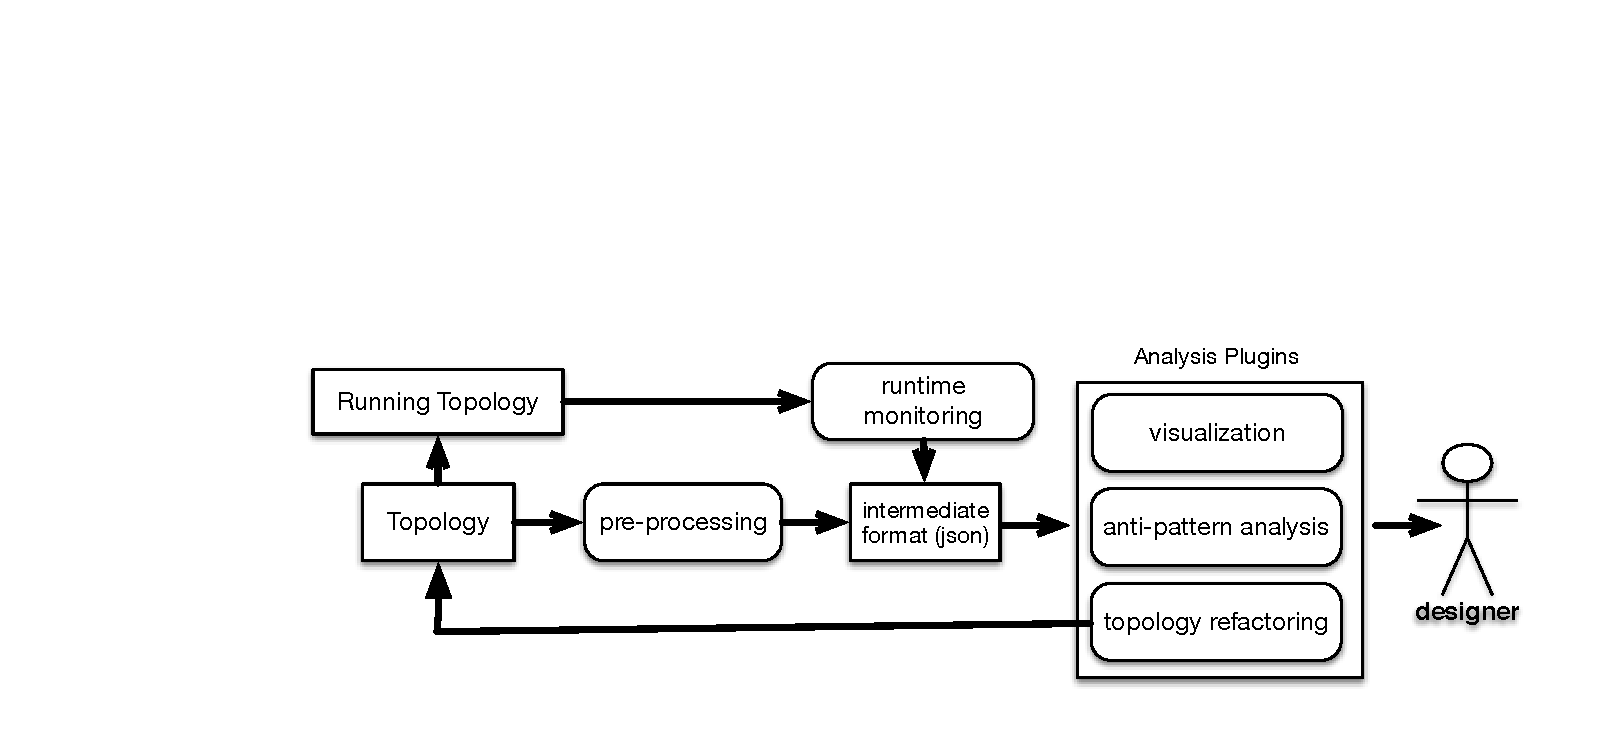
\includegraphics[width=9cm]{images/ostia-arch}
		\caption{OSTIA extensible architecture.}\label{archostia}
	\end{center}
\end{figure}

Such information will be continuously added to the intermediate repository via
runtime monitoring of the topology on real deployment cluster. These provide
appropriate and rich information for refactoring the initial architecture and
enabling performance driven DevOps \cite{brunnert2015performance}.
%%%%%%%%%% COMMENTATO SHORT
%%%%%%%%%%Finally, OSTIA allows users to export the topology in different formats
%%%%%%%%%%(e.g. JSON) to analyse and continuously improve the topology with other tools, e.g., by means of formal verification.

\subsection{Storm Architecture}

Storm is a technology developed at Twitter \cite{toshniwal2014storm} in order to
face the problem of processing of streaming of data. It is defined as a
distributed processing framework which is able to analyse streams of data. The
core element in the system is called \emph{topology}. A Storm topology is a
computational graph composed by nodes of two types: spouts and bolts. The former
type includes nodes that process the data entering the topology, for instance
querying APIs or retrieve information from a message broker, such as Apache
Kafka. The latter executes operations on data, such as filtering or serialising.
%%%%%% COMMENTATO_SHORT
%%%%%%%%%\subsection{Storm Framework Meta-Model}
%%%%%%%%%
%%%%%%%%%OSTIA was designed to retrieve and analyse Storm topologies on-the-fly, allowing their refactoring in a way which is consistent with framework restrictions, rules and regulations part of the Storm framework. To do so, OSTIA uses a meta-model for the Storm framework which acts as an operational image of all said restrictions and rules that OSTIA needs to maintain. 
%%%%%%%%%Essentially OSTIA uses the meta-model as such an operational image for Storm, for two purposes: (a) checking that Storm restrictions (e.g., Spouts initiate the topology) and constraints (e.g., grouping policies) are valid on models recovered by OSTIA; (b) keep checking said restrictions and constraints during continuous architecting. 
%%%%%%%%%The meta-model in question is depicted in Fig. \ref{stormmm}. The figure shows an overview of the meta-model for Storm\footnote{The details of this meta-model and the restrictions captured therein is beyond the scope of this paper. More details are available here: \url{http://dice-h2020.eu/deliverables/D2.1}.} where, for example, the grouping restrictions that Storm envisions are captured in an enumeration of constraints (see the $<<$Grouping$>>$ element or the $<<$ReplicationFactor$>>$ concrete parameter). Key elements of the meta-model are the following:
%%%%%%%%%\begin{itemize}
%%%%%%%%%\item $<<$TopologyConfiguration$>>$ contains the parameters necessary for the Storm framework to be configured and to run on the selected infrastructure. OSTIA checks that these parameters are present or that defaults are correctly inplace;
%%%%%%%%%\item $<<$Topology$>>$ specifies the topological construct being elicited for the analysed Storm application, as composed of the $<<$Bolt$>>$ and  the $<<$Spout$>>$ meta-elements;
%%%%%%%%%\item  $<<$Grouping$>>$ contains restrictions on the possible groupings of the $<<$Bolt$>>$ and the $<<$Spout$>>$ meta-elements within the elicited topology. OSTIA checks these restrictions upon recovery and exporting of topologies;
%%%%%%%%%\end{itemize}
%%%%%%%%%
%%%%%%%%%\begin{figure*}
%%%%%%%%%	\begin{center}
%%%%%%%%%		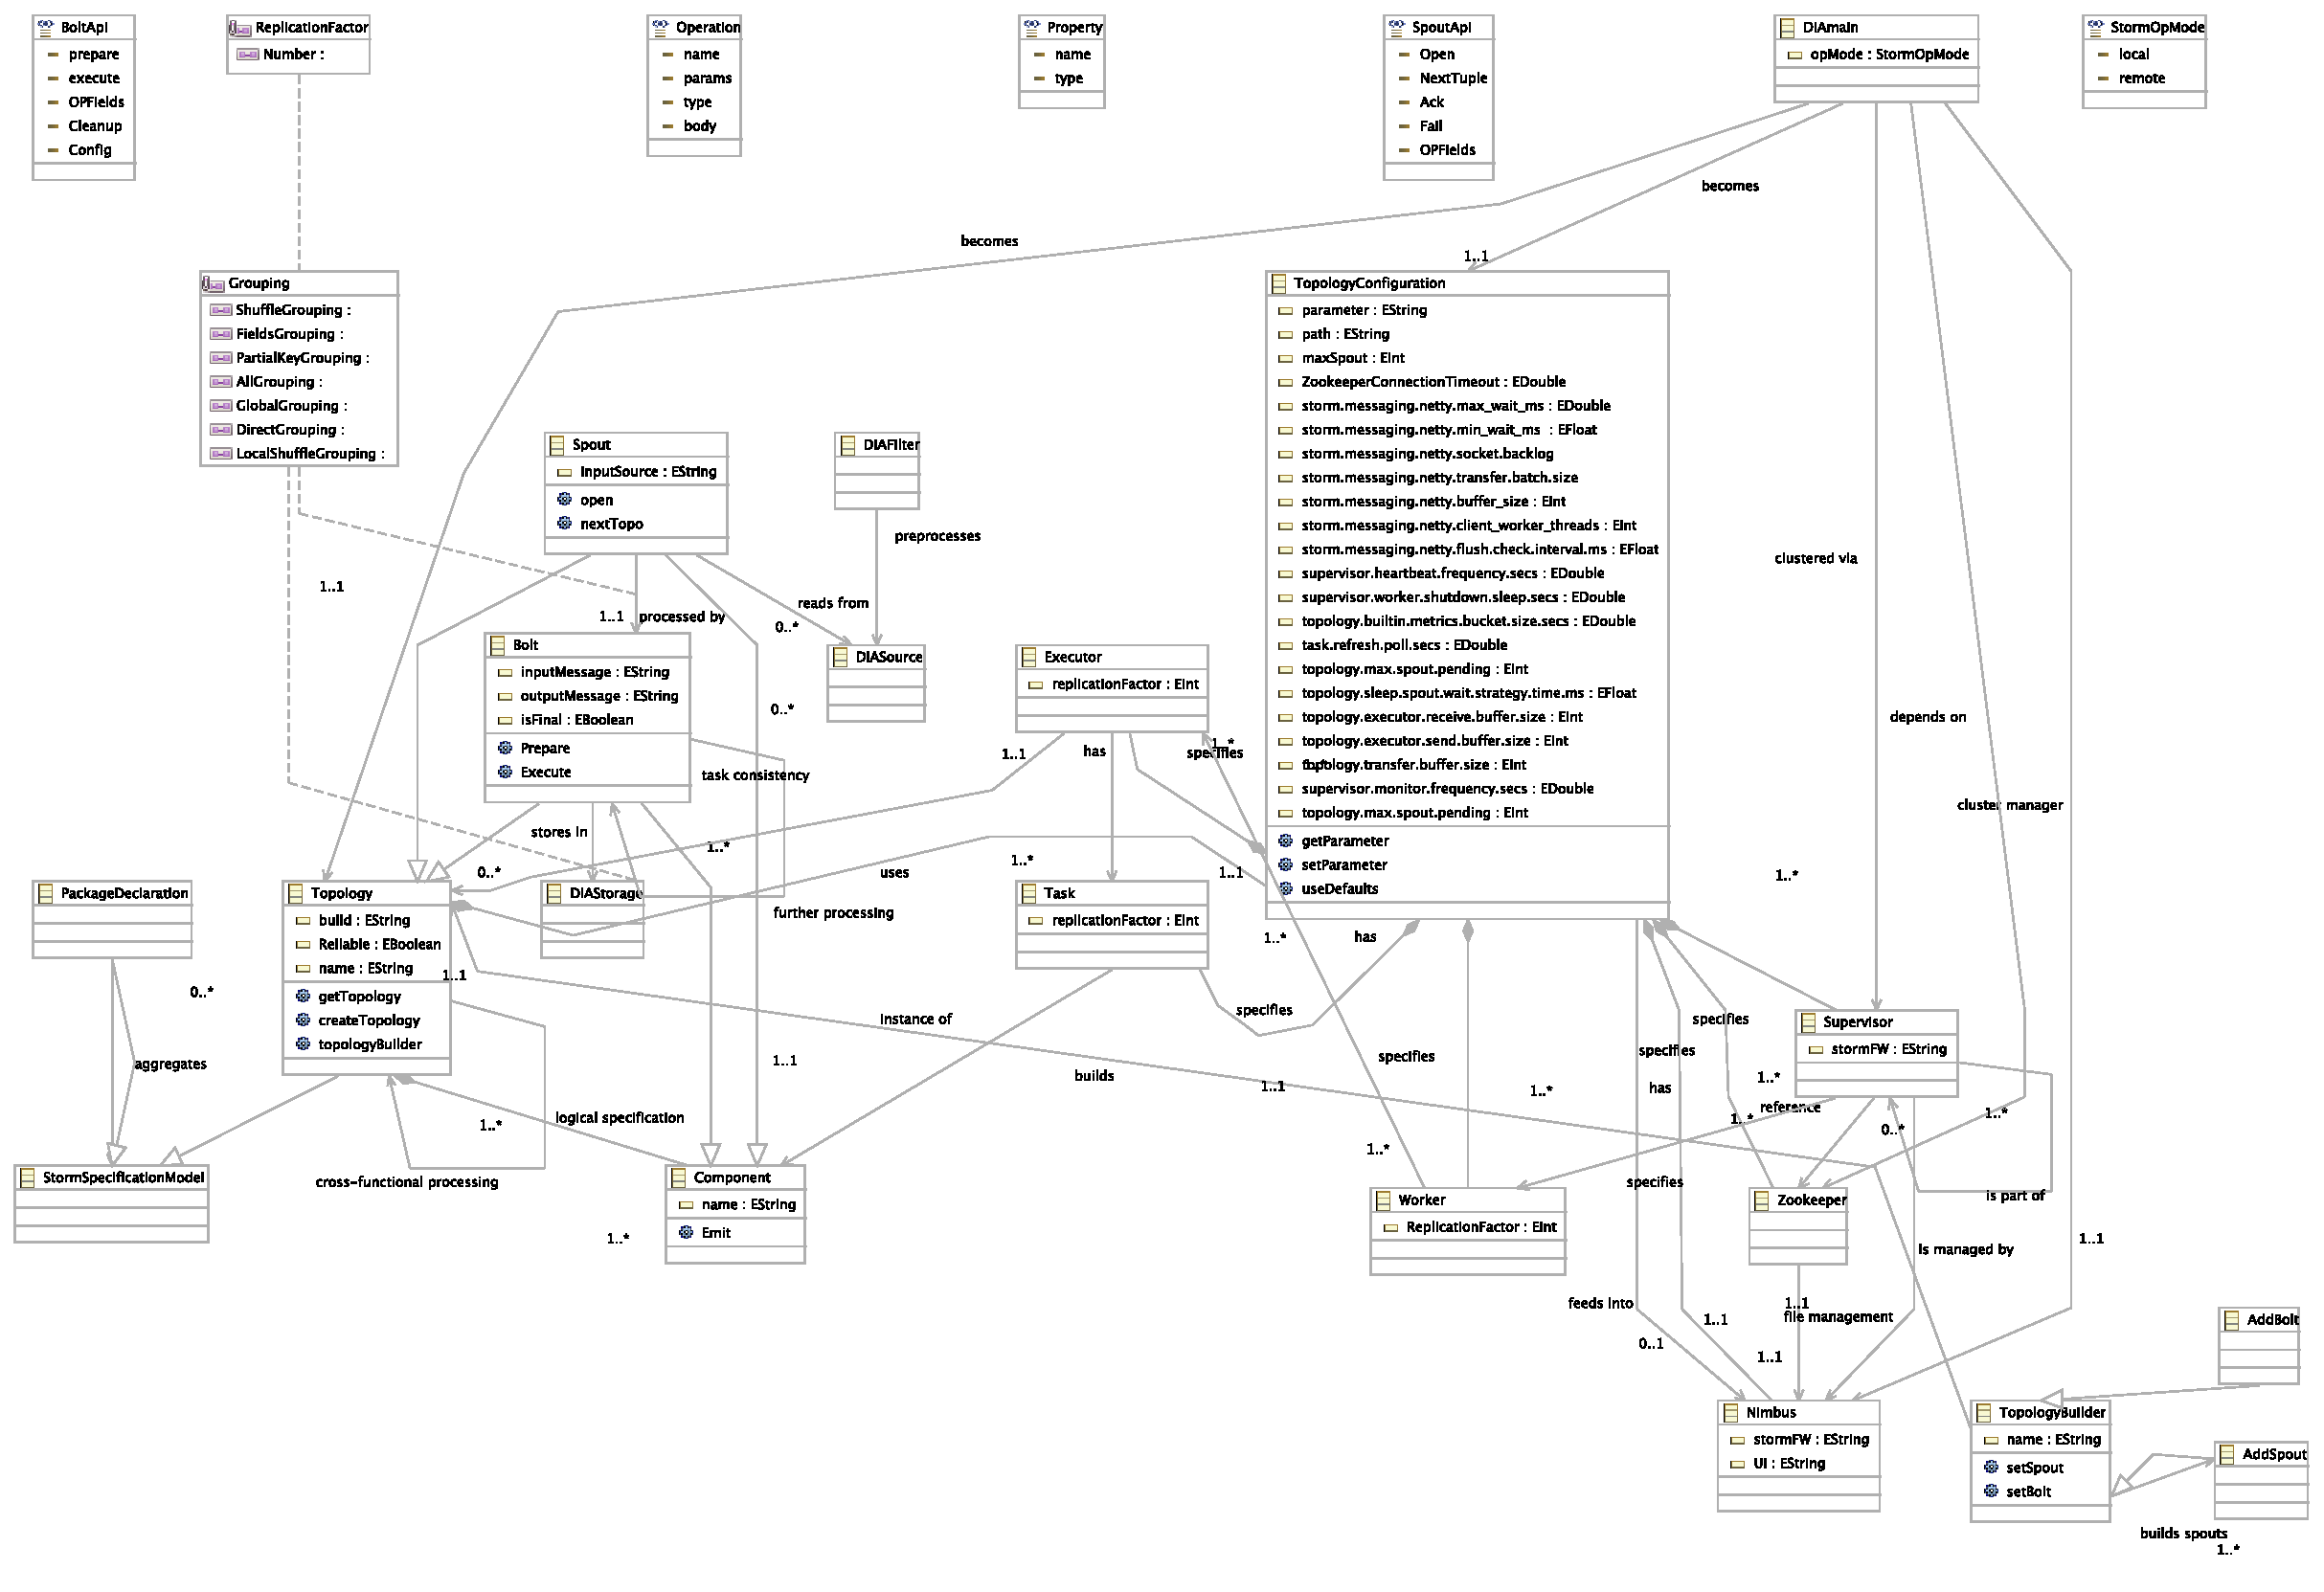
\includegraphics[width=18cm]{images/Stormmm}
%%%%%%%%%		\caption{The Storm Meta-Model.}
%%%%%%%%%		\label{stormmm}
%%%%%%%%%	\end{center}
%%%%%%%%%\end{figure*}
%
%\comment{a description about the verification analyses and more details about the implementations should be added here}
%%%%%% COMMENTATO _ SHORT
%%%%%%%%\subsection{Storm: A Formal Interpretation}
%%%%%%%%Model-checking can serve as a means to enact continuous architecting of Storm topologies. Topologies can undergo formal verification, for example, to assess temporal properties on their execution.
%%%%%%%%This section elaborates on the role of formal verification in OSTIA and describes the necessary background, modelling assumptions and model definition behind Storm topology verification.
%%%%%%%%In particular, we provide a non-deterministic model representing Storm topologies' behavior in terms of the delay connected to bolts' processing, spout input profile and node failures. Spout input profile is measured with rates of incoming tuples into the topology.
%%%%%%%%Verification in OSTIA is intended to discover possible design errors at design time which are caused by (i) under/over estimation of timing requirements of computational nodes or (ii) possible runtime node failures.
%%%%%%%%Therefore, in this context, we are interested in verifying properties like, for instance, the existence of an execution of the topology which guarantees queue-length boundedness even if failures occur with a certain delay.
%%%%%%%%Defining the formal model, requires the comprehension of %started by understanding and capturing 
%%%%%%%%the behaviors of both spouts and bolts which, after choosing the level of abstraction of the model, allows us to abstract those behaviors accordingly, %in order 
%%%%%%%%to formalize them as finite state machines. The purpose of this activity is defining the %possible 
%%%%%%%%operations performed by nodes and their allowed orderings in a real implementation. %of such operations.
%%%%%%%%We then extend the model %by taking into account 
%%%%%%%%considering the message buffers (or queues) and the quantity of tuples that are exchanged through the topology.
%%%%%%%%In addition, %to the correct ordering of the operations, we decided to 
%%%%%%%%we introduce more specific temporal constraints %into the model, in order 
%%%%%%%%to limit the time spent by the system in each state (or processing phase) and to elaborate the concept of \textit{rate}, intended as ``number of times an event is occurring every time unit''.
%%%%%%%%The formal modeling (see Section \ref{ver}) is based on real-time temporal logic, i.e., the topology behavior is defined through a temporal logic formula written in Constraint LTL over clocks (CLTLoc)~\cite{BRS15}.
%%%%%%%%
\label{rs}

\section{OSTIA-Based Continuous Architecting}
This section elaborates on the ways in which OSTIA supports continuous
architecting. First, we elaborate on the anti-patterns supported in
OSTIA. Second, we elaborate on the algorithmic manipulation that OSTIA could
apply to topologies to provide alternative visualisation. Third, we discuss how
OSTIA suggests an alternative architecture to improve the system
performance. Finally, we elaborate on how OSTIA can drive continuous
improvement assisted by formal verification. All figures in these sections use a
simple graph-like notation where nodes may be any topological element (e.g.,
Spouts or Bolts in Apache Storm terms) while edges are directed data-flow
connections.


\subsection{Topology Design Anti-Patterns Within OSTIA}\label{sec:anti-pattern}
This section elaborates on the anti-patterns we elicited through self-ethnography (See Section \ref{ra}). These anti-patterns are elaborated further within OSTIA to allow for their detection during streaming topology inference analysis. Every pattern is elaborated using a simple graph-like notation where \emph{spouts} are nodes that have outgoing edges only whereas \emph{bolts} are nodes that can have either incoming or outgoing edges.

\subsubsection{Multi-Anchoring}
The Multi-Anchoring pattern is shown in Fig. \ref{fig:multi-anchoring}. In order to guarantee fault-tolerant stream processing, tuples processed by bolts need to be anchored with the unique {\sf id} of the bolt and be passed to multiple acknowledgers (or ``ackers" in short) in the topology. In this way, ackers can keep track of tuples in the topology. Multiple ackers can indeed cause much overhead and influence the operational performance of the entire topology.
%\emph{\bf TODO: what is the consequence of these anti-patterns? How does OSTIA detect?}
%\emph{\bf Multi-anchoring is not supported at the moment. Besides, I am not sure it is an anti-patter but rather a design decision}

%\begin{figure}[H]
%	\begin{center}
%		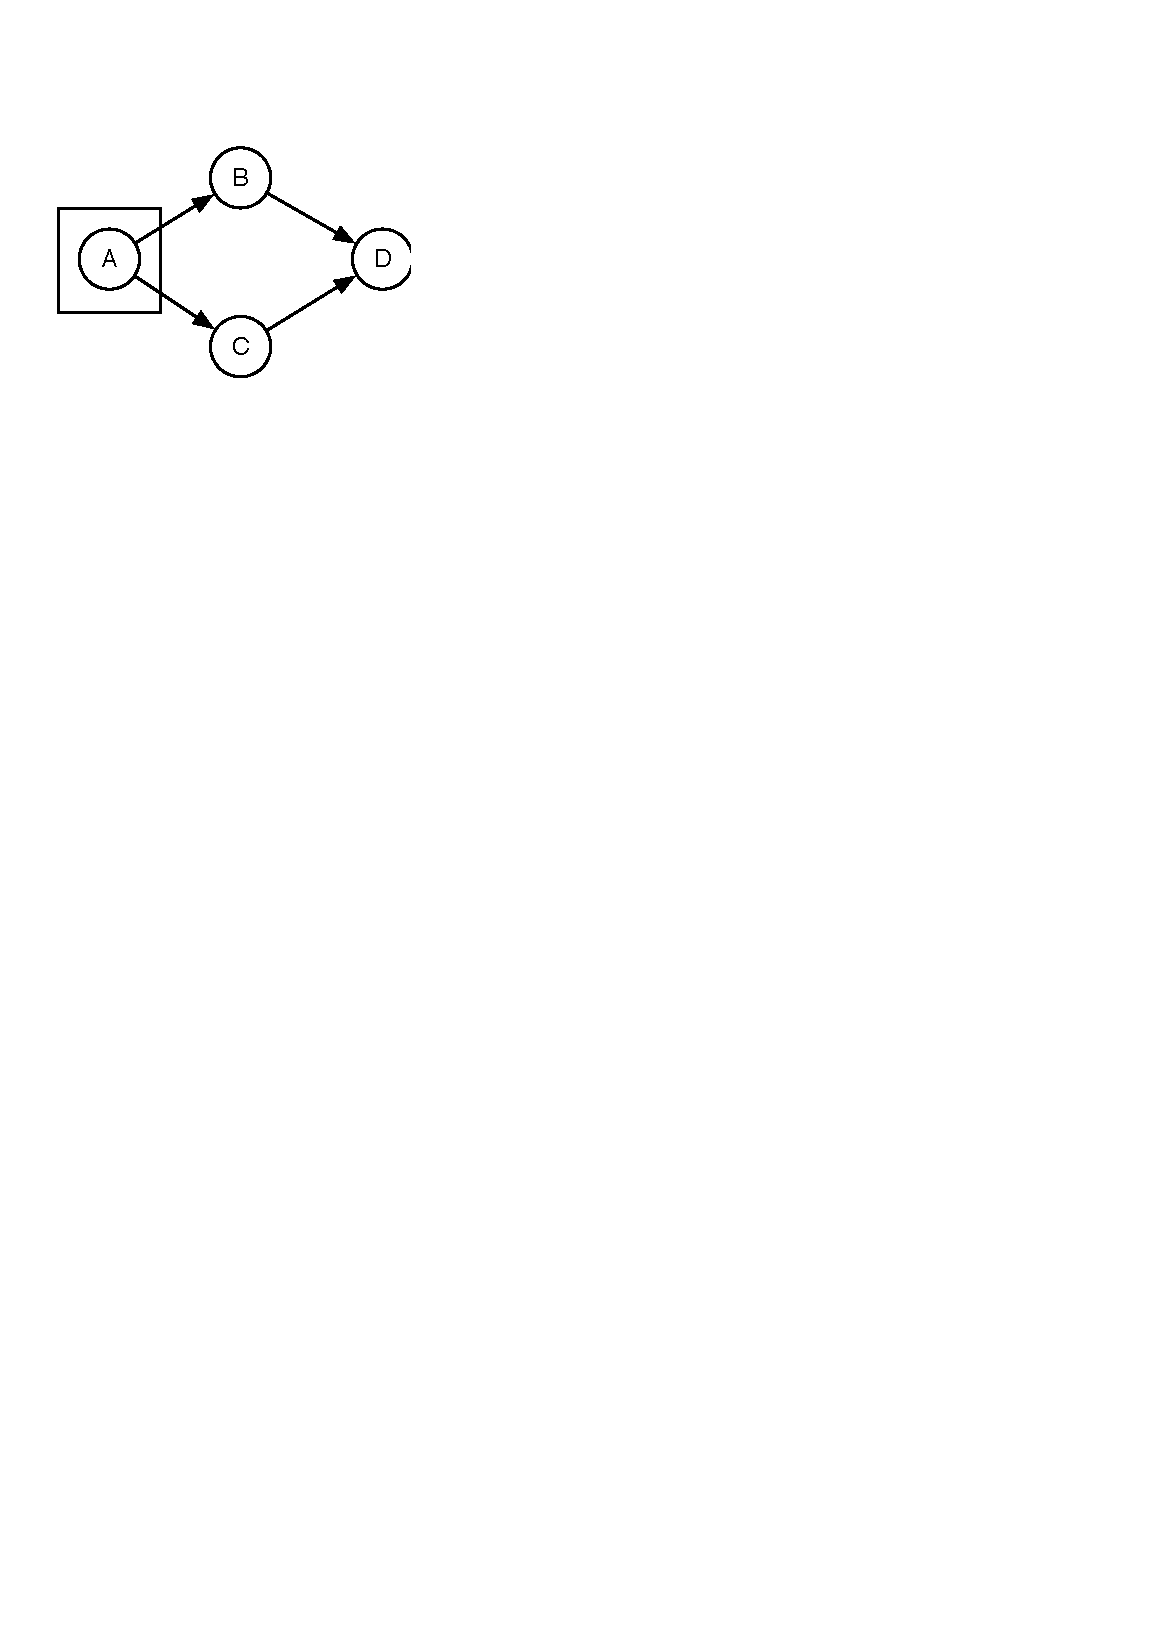
\includegraphics[width=2.5cm]{images/multi-anchoring}
%		\caption{Multi-anchoring.}
%		\label{fig:multi-anchoring}
%	\end{center}
%\end{figure}

\begin{figure}
\centering 
\subfigure[Multi-anchoring.]{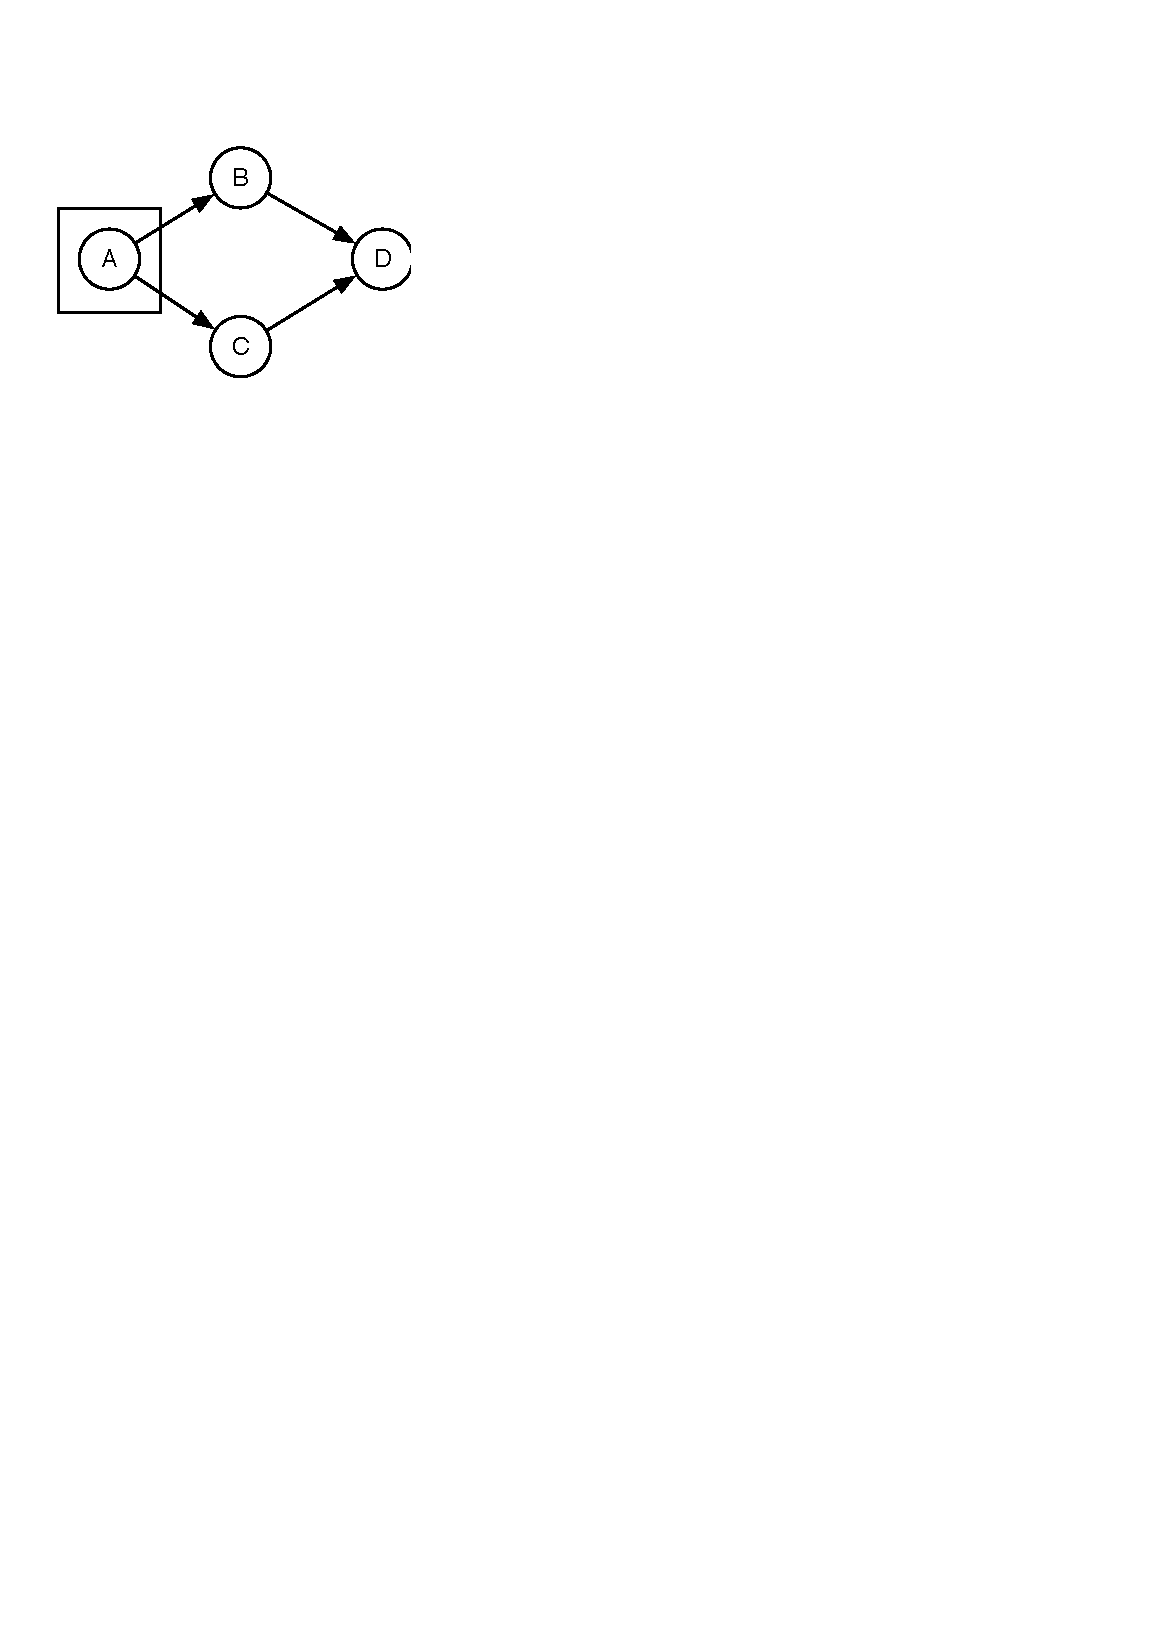
\includegraphics[width=3cm]{images/multi-anchoring}}\label{fig:multi-anchoring}
\hspace{1cm}
\subfigure[Cycle-in.]{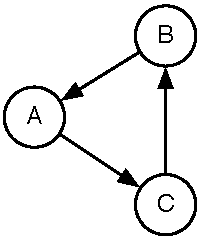
\includegraphics[width=2.5cm]{images/cycle}}\label{fig:cycle}
\end{figure}


\subsubsection{Cycle-in Topology}

The Cycle-in pattern is shown in Fig. \ref{fig:cycle}. Technically, it is possible to have cycle in Storm topologies. An infinite cycle of processing would create an infinite tuple tree and make it impossible for Storm to ever acknowledge spout emitted tuples. Therefore, cycles should be avoided or resulting tuple trees should be investigated additionally to make sure they terminate at some point and under a specified series of conditions (these conditions can be hardcoded in Bolt logic). The anti-pattern itself may lead to infrastructure overloading and increased costs.
%\emph{\bf A topology is already an infinite stream of tuple, the problem could be the overloading of some machines}
%\emph{\bf At the cycle-detection is not supported (even if it is easy to implement)}

%\begin{figure}[H]
%	\begin{center}
%		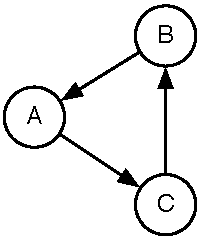
\includegraphics[width=2cm]{images/cycle}
%		\caption{Cycle-in Topology.}
%		\label{fig:cycle}
%	\end{center}
%\end{figure}

\subsubsection{Persistent Data}

The persistent data pattern is shown in Fig. \ref{fig:persistence}. This pattern covers the circumstance wherefore if two processing elements need to update a same entity in a storage, there should be a consistency mechanism in place. OSTIA offers limited support to this feature, which we plan to look into more carefully for future work. More details on this support are discussed in the approach limitations section.
%\emph{\bf Ostia does not support this. BTW is this static analysis? if not, is it off-topic?}

\begin{figure}
	\begin{center}
		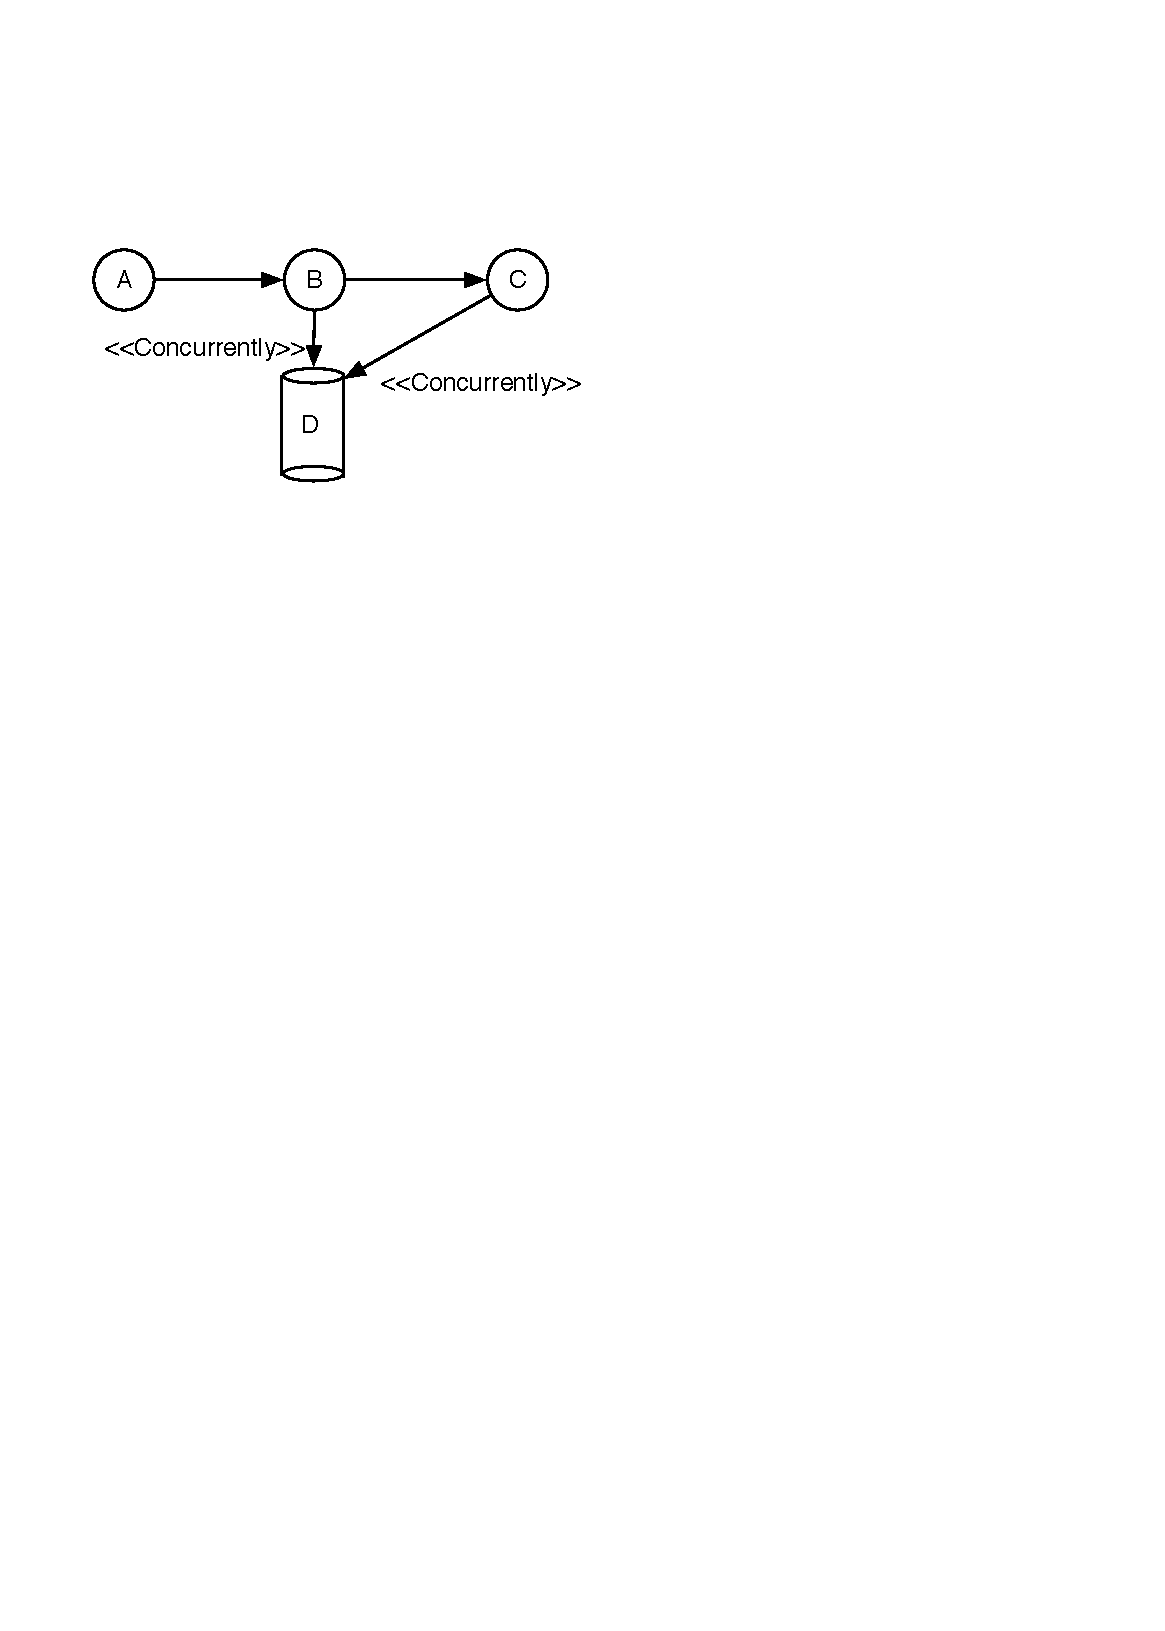
\includegraphics[width=5cm]{images/persistence}
		\caption{Concurrency management in case of Persistent Data circumstances.}
		\label{fig:persistence}
	\end{center}
\end{figure}


\subsubsection{Computation Funnel}
The computational funnel is shown in Fig. \ref{fig:funnel}. A computational funnel emerges when there is not a path from data source (spout) to the bolts that sends out the tuples off the topology to another topology through a messaging framework or through a storage. This circumstance should be dealt with since it may compromise the availability of results under the desired performance restrictions.

\begin{figure}
	\begin{center}
		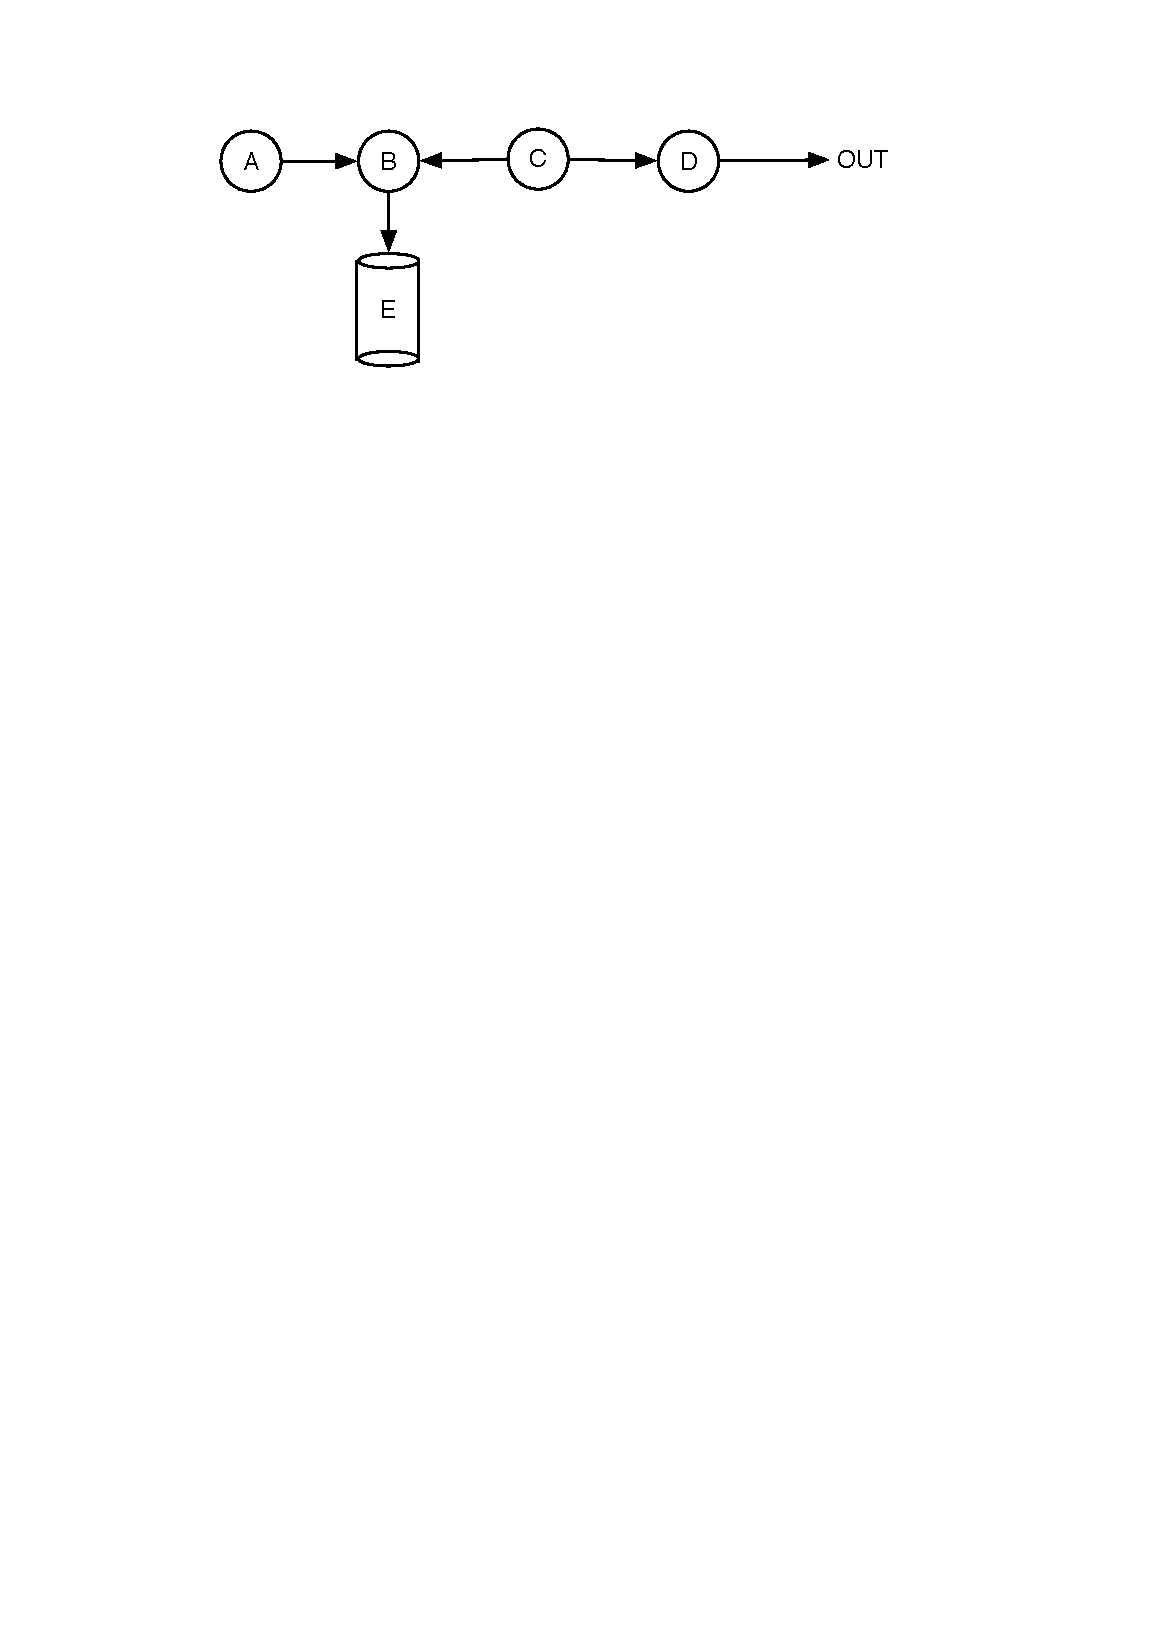
\includegraphics[width=6.5cm]{images/funnel}
		\caption{computation funnel.}
		\label{fig:funnel}
	\end{center}
\end{figure}

\subsection{Algorithmic Analysis on Stream Topologies}\label{algo}

This section elaborates on the algorithmic analysis supported by OSTIA using the common graph-like notation introduced previously. OSTIA currently supports two topology content analysis (see Sec. \ref{1} and \ref{2}) as well as two topology layout analyses (see Sec. \ref{3} and \ref{4}). Only a part of these analyses is currently implemented in OSTIA. We discuss approach limitations further in Sect. \ref{disc}.

\subsubsection{Fan-in/Fan-out}\label{1}

The Fan-in/Fan-out algorithmic manipulation is outlined in Fig. \ref{fig:fan}. For each element of the topology, fan-in is the number of incoming
streams. Conversely, fan-out is the number outgoing streams. In the case of
bolts, both in and out streams are internal to the topology. For Spouts,
incoming streams are the data sources of the topology (e.g., message brokers,
APIs, etc) which live outside of the topology.

\begin{figure}
	\begin{center}
		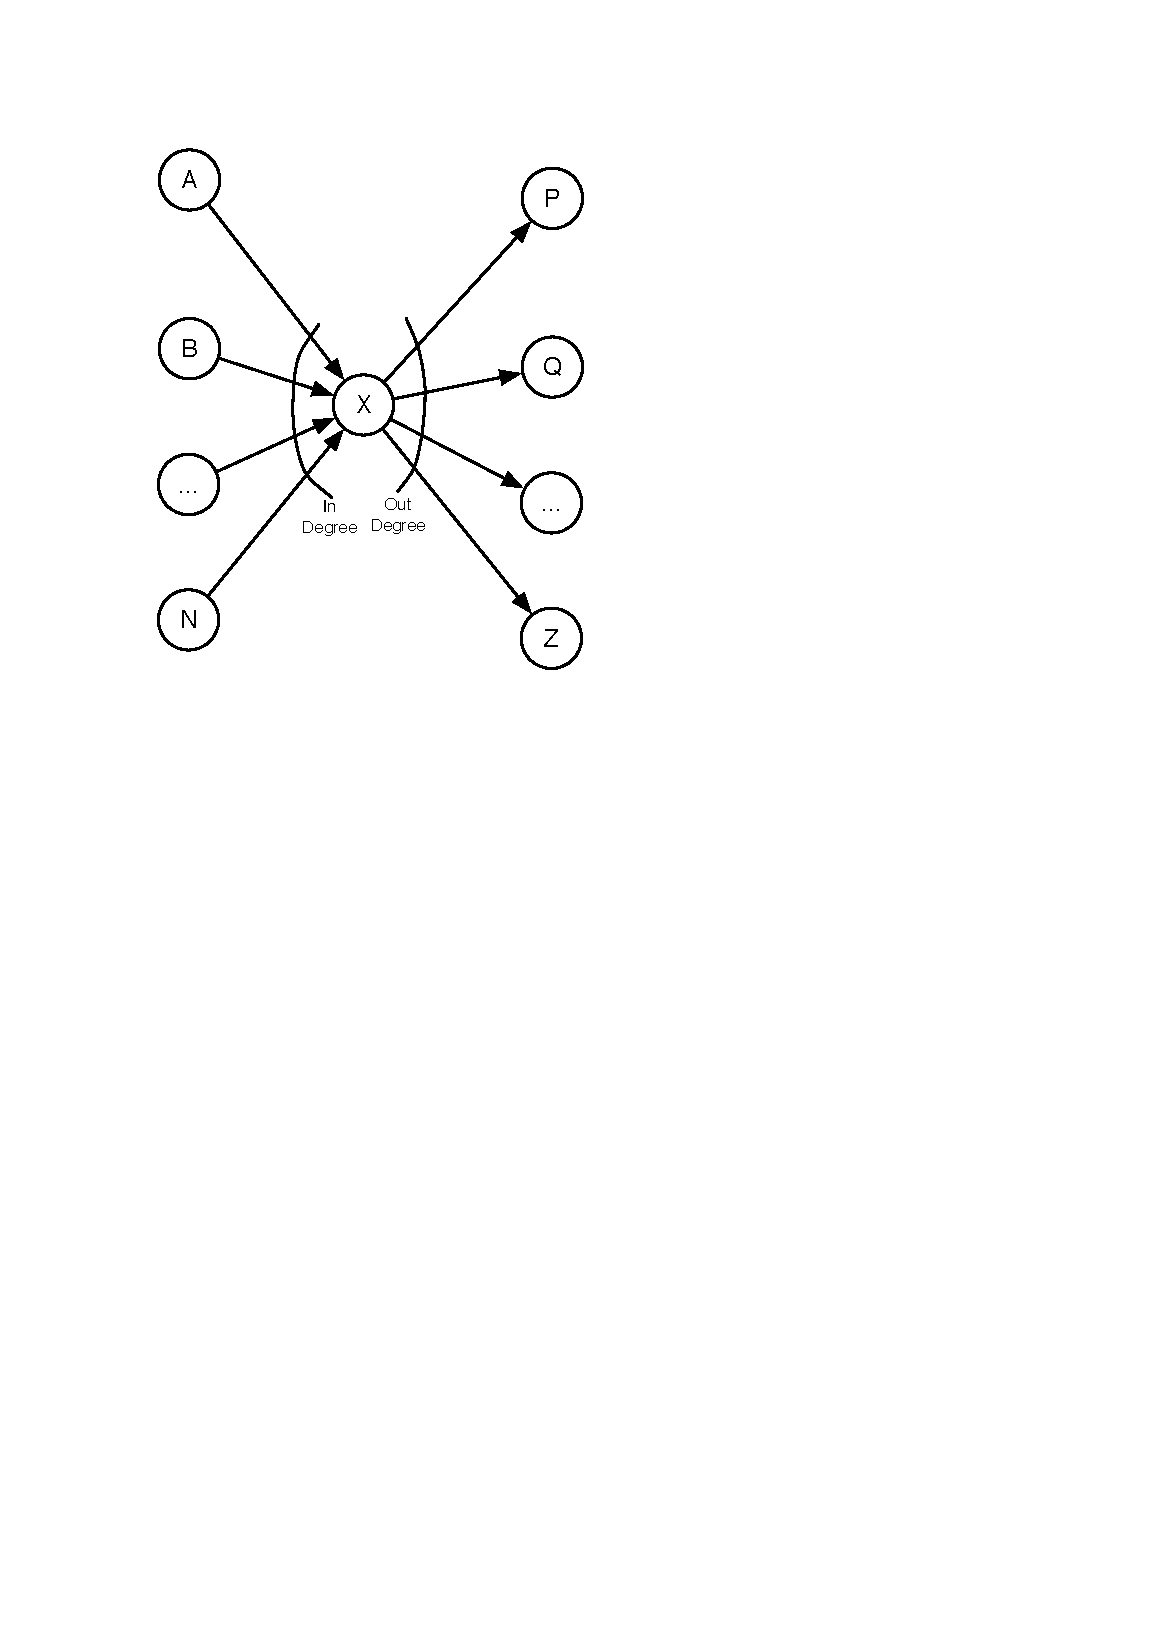
\includegraphics[width=3cm]{images/fan-in-out}
		\caption{Fan-in fan-out in Stream topologies.}
		\label{fig:fan}
	\end{center}
\end{figure}

This algorithmic manipulation allows to visualise instances where fan-in and fan-out numbers are differing.

\subsubsection{Topology cascading}\label{2}

The Cascading algorithmic manipulation is outlined in Fig. \ref{fig:cascading}. By topology cascading, we mean connecting two different Storm topologies via a messaging framework (e.g., Apache Kafka~\cite{kafka}).
%\footnote{\url{http://kafka.apache.org/}}). 
Although cascading may simplify the development of topologies by encouraging architecture elements' reuse especially for complex but procedural topologies, this circumstance may well raise the complexity of continuous architecting and may require separation of concerns \cite{soc}. For example, Fig. \ref{fig:cascading} outlines an instance in which two topologies are concatenated together by a message broker. In this instance, formal verification may be applied on the left-hand side topology, which is more business-critical, while the right-hand side of the entire topology is improved by on-the-fly OSTIA-based analysis. Even though OSTIA support for this feature is still limited, we report it nonetheless since OSTIA was engineered to address multiple topologies at once. 
%More details on this and similar limitations are discussed in Section \ref{lim}.
%\emph{\bf Ostia does not support this. I can't think of an easy way to implement it}

\begin{figure}
	\begin{center}
		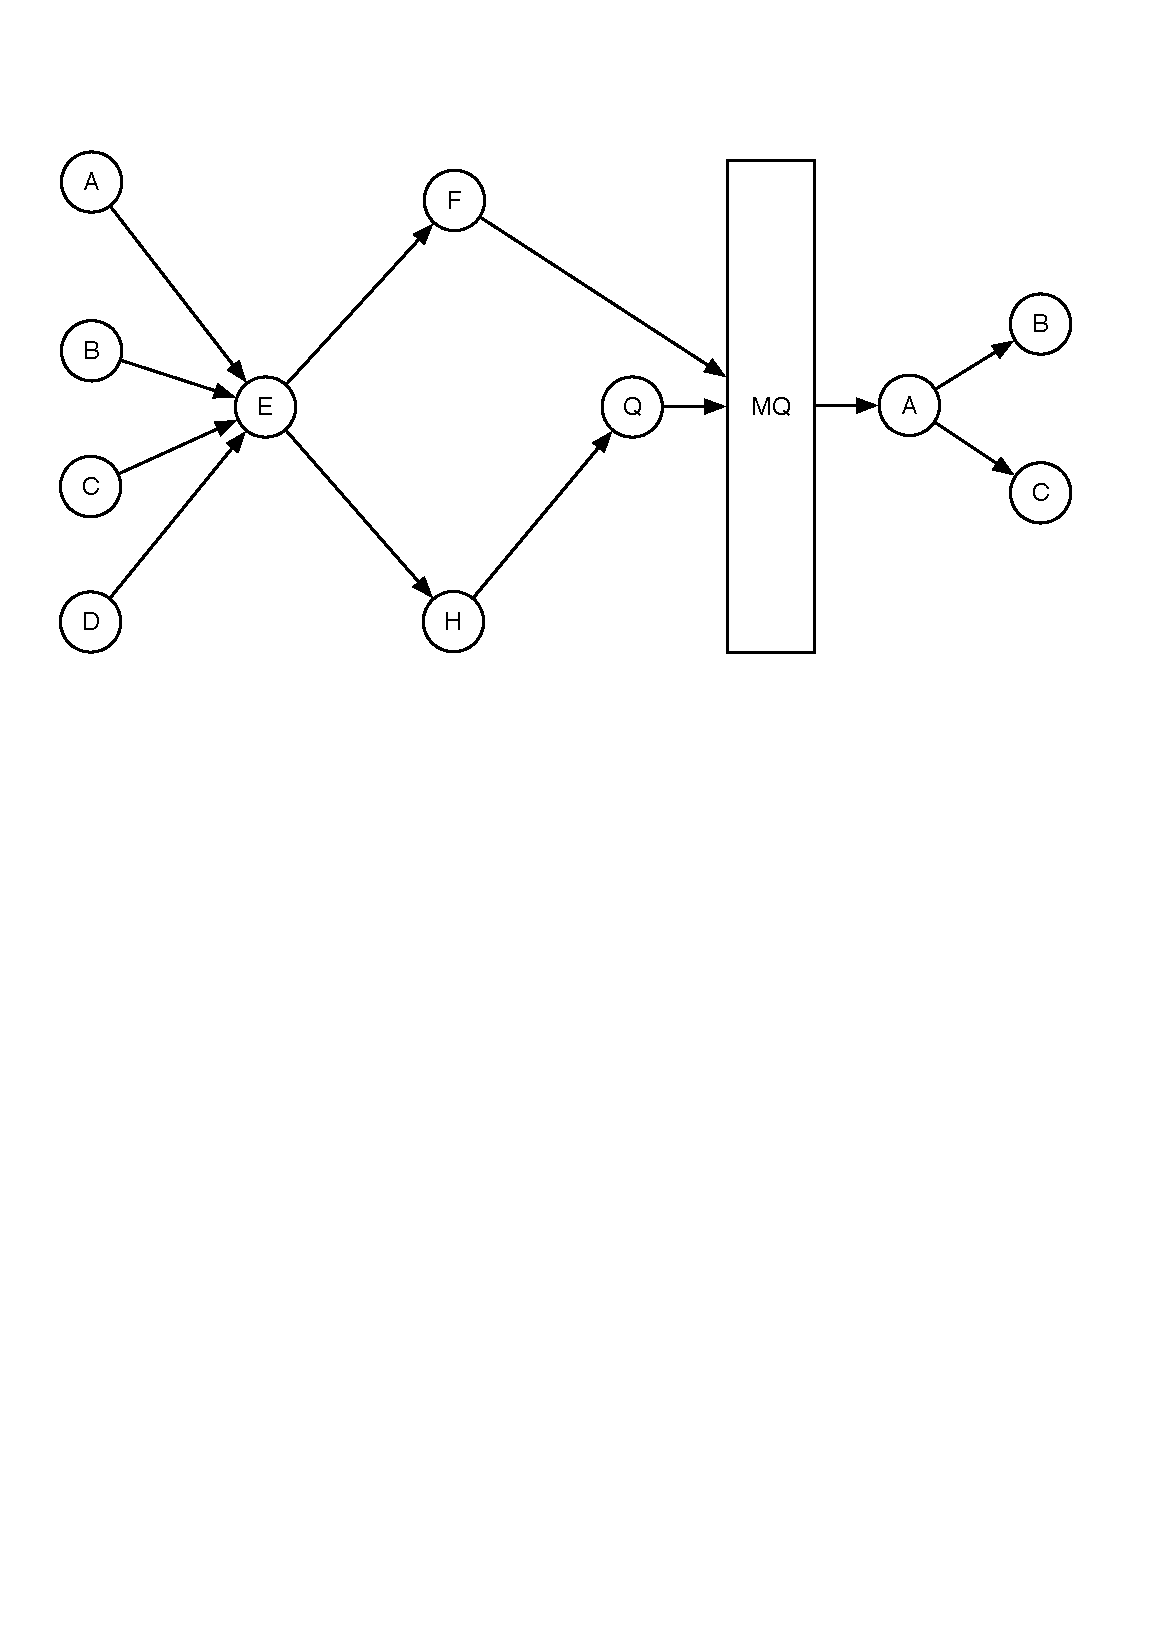
\includegraphics[width=6cm]{images/cascading}
		\caption{cascading.}
		\label{fig:cascading}
	\end{center}
\end{figure}

This algorithmic manipulation allows to combine multiple cascading topologies.

\subsubsection{Topology clustering}\label{3}
Topology clustering is outlined in Fig. \ref{fig:clustering}. Topology clustering implies identifying coupled processing elements (i.e., bolts and spouts) and cluster them together (e.g., by means of graph-based analysis) in a way that elements in a cluster have high cohesion and loose-coupling with elements in other clusters. Simple clustering or Social-Network Analysis mechanisms can be used to infer clusters. These clusters may require additional attention since they could turn out to become bottlenecks. Reasoning more deeply on clusters and their resolution may lead to establishing the Storm scheduling policy best-fitting with the application. We will elaborate on this in Section \ref{sec:performance-boosting}.
%\emph{\bf Does it relates with Storm scheduling?}

\begin{figure}
	\begin{center}
		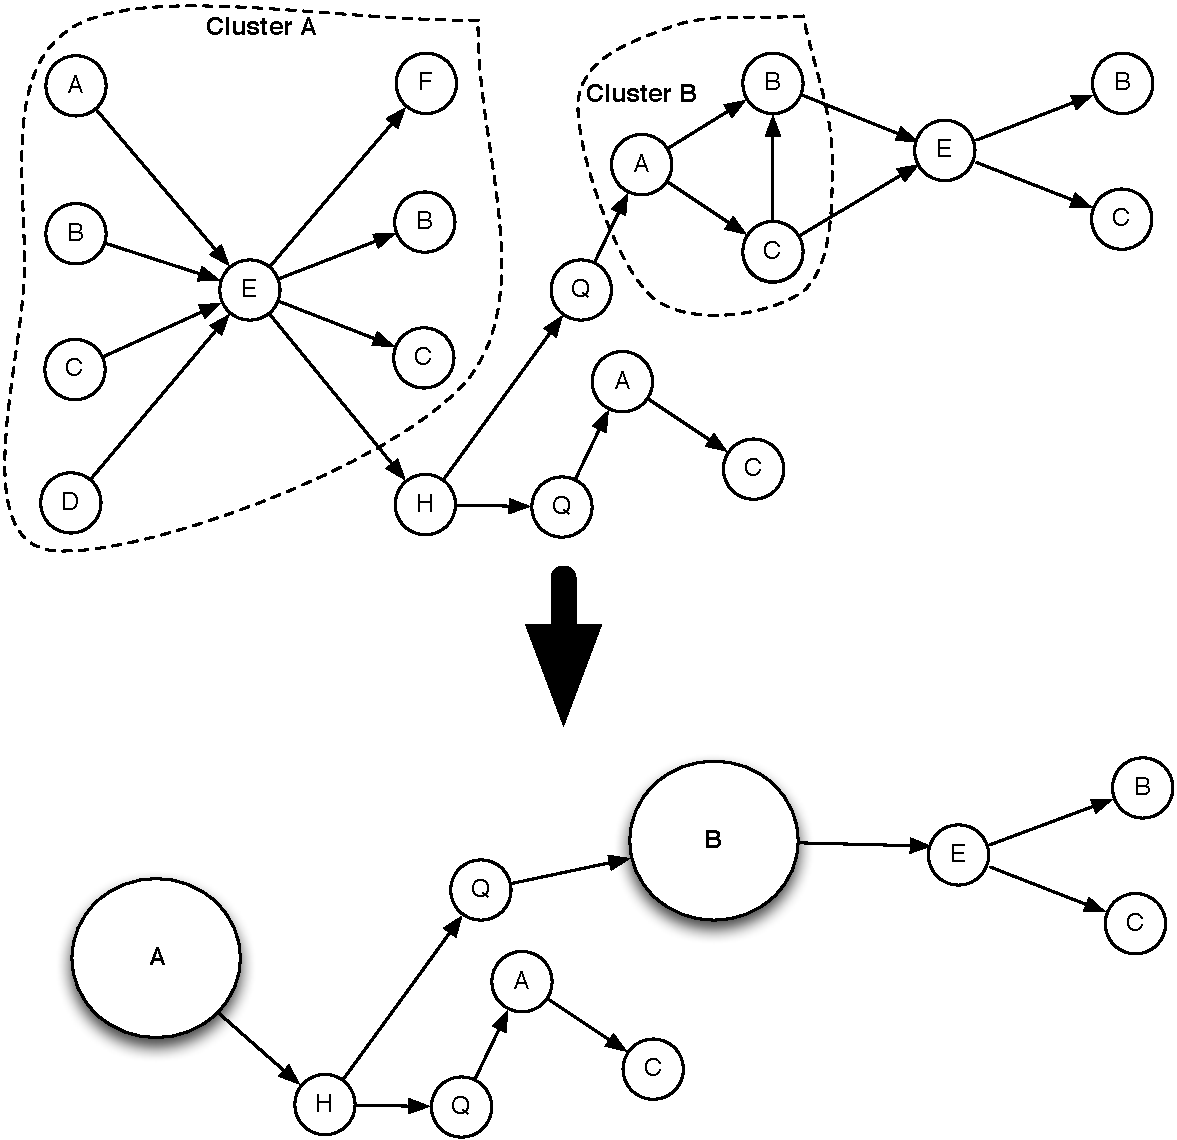
\includegraphics[width=6.5cm]{images/clustering}
		\caption{clustering.}
		\label{fig:clustering}
	\end{center}
\end{figure}

\subsubsection{Linearising a topology}\label{4}

Topology linearisation is outlined in Fig. \ref{fig:linearizing}. Sorting the processing elements in a topology in a way that topology looks more linear, visually. This step ensures that visual investigation and evaluation of the structural complexity of the topology is possible by direct observation. It is sometimes essential to provide such a visualisation to evaluate how to refactor the topology as needed.

\begin{figure}
	\begin{center}
		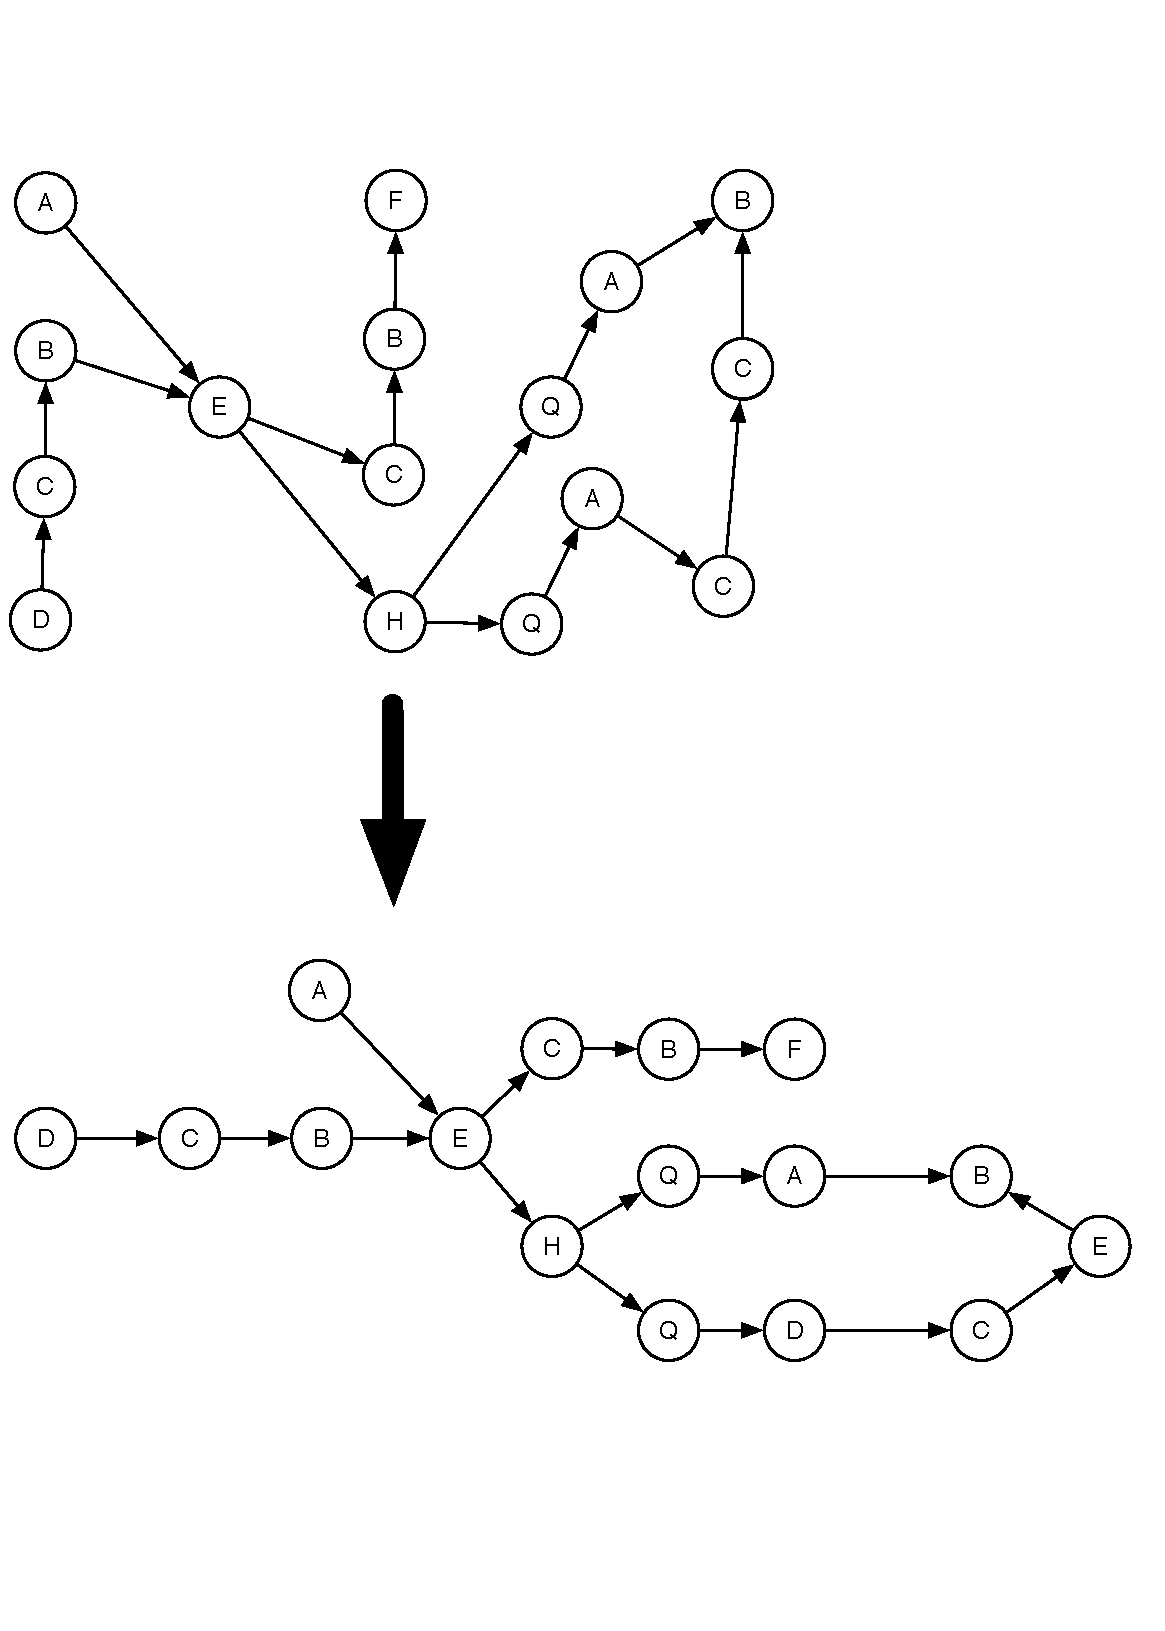
\includegraphics[width=5cm]{images/linearizing}
		\caption{linearising.}
		\label{fig:linearizing}
	\end{center}
\end{figure}

\subsection{Performance Improvement Heuristics}
\label{sec:performance-boosting}
In this section, we elaborate on a specific case where algorithmic analysis on the Stream topology can help to improve the performance of the Stream processing system.

Big data architectures typically need parameters tuning to achieve best
performance. For instance, in Storm developers have to specify the parallelism
level for each node, which is the number of processes instantiated for a
particular bolt or spout. OSTIA provides suggestions on how to change the
parallelism level of the nodes, using simple and fast heuristics together with
static analysis.

After architects designed a Storm application, a scheduler instantiate the
topology on a cluster of machines. The default scheduler utilises a round-robin
strategy to fairly load the machines with the bolts and spouts. This a crucial
assumption for the heuristic used in OSTIA to perform well. There has been some
proposal to change the default scheduler logic in order to boost the performance
of the topologies \cite{Aniello2013Adaptive, R-Storm2015Peng}. However, many
Storm users typically prefer the default scheduler, while having the opportunity
to tune the parameter automatically behind the scenes.

The heuristic works as follow. A Storm architect runs OSTIA specifying the
number of machines used in the deployment and the number of instances of spouts
and bolts that can be spawned in each machine. OSTIA statically analyses the
topology and extract the parallelism level for each component of the
topology. At this point, we sum of all instances need to be allocated and the
slots available on the machines ($machines * components\_for\_each\_machine$).

OSTIA decides whether a possible improvements is possible (i.e. \emph{slots
  available} $>$ \emph{instances to be allocate}), and suggests changes to the
parallelism level to the nodes in order to improve the performance. The simplest
case occur when the unallocated slots are enough to remove a machine from the
cluster, thus saving costs.

Alternatively, OSTIA identify a subset of nodes, called critical nodes, which
are important from a performance perspective. The critical nodes of a topology
are defined as the nodes with the highest \emph{weighted fan-in}. The
\emph{weighted fan-in} of a node \emph{N} is defined by Equation \ref{eq:wfi}.

\begin{align}
  \text{weighted fan-in(N)} = \frac{\sum_{X \rightarrow N \in Edges} parallelism(X)}{parallelism(N)} \label{eq:wfi}
\end{align}

The critical nodes could be easily susceptible to overloading as their
parallelism level do not compensate the parallelism level of its
\emph{in-nodes}. Increasing the parallelism level gives the nodes more resources
to cope with high loads.

For instance, let us take Figure \ref{topo1} as an example. There are 22
components that need to be allocated. Suppose that our cluster is composed by 4
machines and each machine fits 10 instances of components. OSTIA in this case
would suggest to simply remove one machine. Let us suppose that we have 3
machines with 10 tasks each. At this point we have 30 slots available and 22
components, therefore we have 8 slots available that can be used to increase the
performance. In order to decide the components to improves we identify the ones
with maximum \emph{weighted fan-in}. In the example nodes \emph{mediaExtractor}
and \emph{articleExtractor} with \emph{weighted fan-in} of 8. Finally, since we
have 8 free slots to share between two nodes we increase the parallelism level
of the two critical nodes of $8/2 = 4$, setting it from 1 to 5.

The above heuristic approach concludes the support that OSTIA offers to quickly and continuously improving streaming topologies by means of algorithmic evaluations and manipulations. Conversely, as previously stated we learned from industrial practice that the need might rise for more formal guarantees, e.g., concerning some key parts of a streaming topology with respect to key big-data properties such as queue-boundedness - i.e., a guarantee that the queue for a certain bolt will always be bounded - or queue-population - i.e., a guarantee that the queue never contains privacy sensitive objects. In similar scenarios, OSTIA offers the seamless capability of running complex and exhaustive formal verification over analysed topologies. The next section elaborates further on this key support offered by OSTIA.

%
%\comment{PJ: Should we put this section into a separate section? I feel it is disconnected to the content of this section.}
\subsection{OSTIA-Based Formal Verification}\label{ver}

\newcommand{\I}{\mathcal{I}}
\newcommand{\M}{\mathcal{M}}
\newcommand{\timestr}{\mathcal{T}}

\newcommand{\D}{\mathcal{D}}
\newcommand{\C}{\mathcal{C}}

%old, compatibility reasons
\newcommand{\U}{\mathbf{U}}
\newcommand{\Snc}{\mathbf{S}}
\newcommand{\T}{\mathbf{T}}
\newcommand{\R}{\mathbf{R}}

\newcommand{\Nat}{\mathbb{N}}
\newcommand{\Z}{\mathbb{Z}}
\newcommand{\Real}{\mathbb{R}}
\newcommand{\Q}{\mathbb{Q}}

%old, compatibility reasons

\newcommand{\X}[1]{\mathbf{X}\left(#1\right)}
\newcommand{\Y}[1]{\mathbf{Y}\left(#1\right)}

%\newcommand{\X}{\mathbf{X}}
%\newcommand{\Y}{\mathbf{Y}}


\newcommand{\Zed}{\mathbf{Z}}
\newcommand{\Lng}{\mathscr {L}}
\newcommand{\iFF}{\Leftrightarrow}
\newcommand{\niFF}{\nLeftrightarrow}
\newcommand{\SNC}{{\mathcal S}}
\newcommand{\TRG}{{\mathcal T}}
\newcommand{\zot}{$\mathds{Z}$ot}
%old, compatibility reasons
\newcommand{\G}[1]{\mathbf{G}\left(#1\right)}
\newcommand{\F}[1]{\mathbf{F}\left(#1\right)}
%\newcommand{\Q}{\mathbb{Q}}

\newcommand{\triple}[3]{(#1, #2, #3)}
\newcommand{\pair}[2]{(#1, #2)}
\newcommand{\siff}{\Leftrightarrow}
\newcommand{\A}{\mathcal{A}}
\newcommand{\aX}{\mathrm{X}}
\newcommand{\aY}{\mathrm{Y}}
\newcommand{\x}{\mathbf{x}}
\newcommand{\eqdef}{\stackrel{\mbox{\begin{tiny}def\end{tiny}}}{=}} % =def=
\newcommand{\iFFdef}{\stackrel{\mbox{\begin{tiny}def\end{tiny}}}{\iFF}}
% =def=
\newcommand{\step}[1]{\xrightarrow{#1}}

\newcommand{\pspace}{\textsc{PSpace}}


\makeatletter
\def\Eqlfill@{\arrowfill@\Relbar\Relbar\Relbar}
\newcommand{\longmodels}[1][]{\,|\!\!\!\ext@arrow 0359\Eqlfill@{#1}}
\makeatother

\newcommand{\symodels}{\longmodels{\mbox{\it{\tiny sym}}}}

\newcommand{\intervaLii}[2]{[#1,#2]}
\newcommand{\intervaLie}[2]{[#1,#2)}
\newcommand{\intervaLee}[2]{(#1,#2)}

\newcommand{\interval}[2]{\langle #1,#2 \rangle}

\newcommand{\set}[1]{\{ #1 \}}

\newcommand{\tsys}[1]{\mathcal{S}(#1)}


\newcommand{\lapp}[1]{\lfloor #1 \rfloor}
\newcommand{\happ}[1]{\lceil #1 \rceil}


\newcommand{\first}[2]{(H_{#1}\vee L_{#1}) \wedge(\neg(H_{#1}\vee L_{#1}) \Snc (#2))}



\newcommand{\pname}[1]{\ensuremath{\textit{#1}}}
\newcommand{\on}{\pname{on}}
\newcommand{\off}{\pname{off}}
\newcommand{\lon}{\pname{l}}
\newcommand{\test}{\pname{test}}
\newcommand{\resetc}{\pname{reset-c}}
\newcommand{\turnoff}{\pname{turnoff}}




\newcommand{\edge}[1]{\texttt{#1}}
\newcommand{\enabled}[1]{\texttt{e}_{#1}}

\newcommand{\visit}[1]{\mathit{visit}(#1)}
\newcommand{\inv}[1]{\mathit{inv}(q_{#1})}


\newcommand{\intg}[1]{\lfloor#1\rfloor}
\newcommand{\fract}[1]{\mathit{frac(#1)}}



%%%%%%%%%%%%%%% STORM MODEL COMMANDS


\newcommand{\ori}{\mathtt{orig}}
%commands with single parameter
\newcommand{\p}[1]{\mathtt{process}_{#1}}
\newcommand{\ta}[1]{\mathtt{take}_{#1}}
\newcommand{\e}[1]{\mathtt{emit}_{#1}}
\newcommand{\add}[1]{\mathtt{add}_{#1}}
\newcommand{\f}[1]{\mathtt{fail}_{#1}}
\newcommand{\buf}[1]{\mathtt{buffer}_{#1}}
\newcommand{\startf}[1]{\mathtt{startFailure}_{#1}}
\newcommand{\startid}[1]{\mathtt{startIdle}_{#1}}
\newcommand{\id}[1]{\mathtt{idle}_{#1}}
\newcommand{\cl}[1]{\mathtt{clock}_{#1}}
\newcommand{\cltf}[1]{ \cl{to\f{#1}}}
\newcommand{\ph}[1]{\mathtt{phase}_{#1}}

%commands with two parameters (index, rate)
\newcommand{\pr}[2]{\p{#1}(#2)}
\newcommand{\tar}[2]{\ta{#1}(#2)}
\newcommand{\er}[2]{\e{#1}(#2)}
\newcommand{\addr}[2]{\add{#1}(#2)}
\newcommand{\ra}[1]{r_{\add{#1}}}
\newcommand{\rp}[1]{r_{\p{#1}}}
\newcommand{\re}[1]{r_{\e{#1}}}
\newcommand{\rt}[1]{r_{\ta{#1}}}
\newcommand{\rf}[1]{r_{\mathtt{failure}_{#1}}}
\newcommand{\rff}[2]{r_{\mathtt{failure}_{#1#2}}}
\newcommand{\rr}[1]{r_{\mathtt{replay}_{#1}}}
\newcommand{\reb}[1]{\bar{r}_{\e{#1}}}
\newcommand{\rth}[1]{\hat{r}_{\ta{#1}}}
\newcommand{\reh}[1]{\hat{r}_{\e{#1}}}

\newcommand{\tph}[2]{t_{\ph{#1}}^{#2} }

	

This section describes the formal modelling and verification employed in OSTIA. Our assumption for continuous architecting is that architects eliciting and studying their topologies by means of OSTIA may want to continuously and incrementally improve it based on results from solid verification approaches. The approach, which was first proposed in \cite{MBER16}, relies on \textit{satisfiability checking}~\cite{MPS13}, an alternative approach to model-checking where, instead of an operational model (like automata or transition systems), the system (i.e., a topology in this context) is specified by a formula defining its executions over time and properties are verified by proving that the system logically entails them.

%The logic we use is Constraint LTL over clocks 
CLTLoc is a real-time temporal logic and, in particular, a semantic restriction of Constraint LTL (CLTL)~\cite{DD07} allowing atomic formulae over $(\mathbb{R}, \set{<,=})$ where the arithmetical variables behave like clocks of Timed Automata (TA)~\cite{timed}.
As for TA, clocks measures time delays between events: a clock $x$ measures the time elapsed since the last time when $x=0$ held, i.e., since the last ``reset'' of $x$.
Clocks are interpreted over Reals and their value can be tested with respect to a positive integer value or reset to 0.
%
To analyse anomalous executions of Storm topologies which do not preserve the queue-length boundedness property for the nodes of the application, we consider CLTLoc with counters.
Counters are discrete non-negative variables that are used in our model to represent the length of bolt queues over the time throughout the streaming processing realized by the application.
Let $X$ be a finite set of clock variables $x$ over $\Real$, $Y$ be a finite set of variables over $\Nat$ and $AP$ be a finite set of atomic propositions $p$.
CLTLoc formulae with counters are defined as follows:
\begin{equation*}%\small
  \phi :=
  \begin{gathered}
    p \mid x\sim c \mid y\sim c\mid \aX y\sim z\pm c \mid\phi \wedge \phi \mid \neg \phi \mid \\
       \X{\phi} \mid \Y{\phi} %\mid \Zed\phi
\mid \phi\U\phi \mid \phi\Snc\phi
  \end{gathered}
\end{equation*}
where $x \in X$, $y,z \in Y$, $c \in \Nat$ and 
$\sim \in \set{<,=}$, $\mathbf{X}$, $\mathbf{Y}$, $\U$ and $\Snc$ are the
usual ``next'', ``previous'', ``until'' and ``since''.
%The semantics of CLTLoc is defined with respect to $(\Real, \set{<,=})$ and $\pair{\Nat}{<}$, the latter representing positions in time.
A \textit{model} is a pair $\pair{\pi}{\sigma}$, where $\sigma$ is a mapping associating every variable $x$ and position in $\Nat$ with value $\sigma(i,x)$ and $\pi$ is a mapping associating each position in $\Nat$ with subset of $AP$. 
The semantics of CLTLoc is defined as for LTL except for formulae $x\sim c$ and $\aX y \sim z\pm c$. 
%At position $i\in\Nat$, $ \pair{\pi}{\sigma}, i \models x\sim c \textbf{ iff }  \sigma(i, x)\sim c$ and $\pair{\pi}{\sigma}, i \models \aX y\sim z \pm c \textbf{ iff }  \sigma(i+1, z) \sim \sigma(i,z) \pm c$.
Intuitively, formula $x\sim c$ states that the value of clock $x$ is $\sim$ than/to $c$ and formula $\aX y \sim z\pm c$ states that the next value of variable $y$ is $\sim$ to/than $z+c$.

The standard technique to prove the satisfiability of CLTL and CLTLoc formulae is based on of B\"uchi automata \cite{DD07,BRS15} %the evidence has turned out that it may be rather expensive in practice, even in the case of LTL (the size of the automaton is exponential with respect to the size of the formula).
but, for practical implementation, Bounded Satisfiability Checking (BSC)~\cite{MPS13} avoids the onerous construction of automata by means of a reduction to a decidable Satisfiability Modulo Theory (SMT) problem~\cite{BRS15}.
%By unrolling the semantics of a formula for a finite number $k>0$ of steps, 
The outcome of a BSC problem is either an infinite ultimately periodic model or unsat.
%\cite{BRS15} shows that BSC for CLTLoc is complete and that is reducible to a decidable Satisfiability Modulo Theory (SMT) problem. 
%A CLTLoc formula can be translated into the decidable theory of quantifier-free formulae with equality and uninterpreted functions combined with the theory of Reals over $(\Real,<)$. %, written QF-EUF$(\Real,<)$.

CLTLoc allows the specification of non-deterministic models using temporal constraints wherein clock variables range over a dense domain and whose value is not abstracted.
Clock variables represent, in the logical language and with the same precision, physical (dense) clocks implemented in real architectures.
%They appear in formulae in the form $x \sim c$ to express a bound $c$ on the delay measured by clock $x$. 
Clocks are associated with specific events to measure time elapsing over the executions.
As they are reset when the associated event occurs, in any moment, the clock value represents the time elapsed since the previous reset and corresponds to the elapsed time since the last occurrence of the event associated to it.
We use such constraints to define, for instance, the time delay required to process tuples or between two node failures.\\

%Modeling topologies requires to express by formulae emitting rates which measure the number of tuples emitted by a spout node per time unit.
%***TBC

%Verification techinques:
%\begin{itemize}
%\item Safety Verification
%\item Performance analysis	
%\end{itemize}
%A \textit{safety} property is intuitively defined in the formal verification context as a property stating that something ``bad'' will \textit{never} happen during execution.\cite{lamport1}
%Cassical examples of safety properties are deadlock freedom and mutual exclusion, where the ``bad'' behaviour is respectively the deadlock occurrence and the simultaneous execution of a critical section.
%One of the most important requirements for streaming systems is guaranteeing low latency while maintaining high throughput. 
%In a distributed  --> Motivare questione delle code!
%

%
%\subsection{Storm Formal Model}
%\label{sec:storm-model}
%To perform our verification tasks we defined a formal model expressed in CLTLoc with discrete variables. The resulting model is a non-deterministic infinite state system.

% MOVED BEFORE
%%%\subsubsection{OSTIA Models: a Formal Interpretation}
%%%We started by understanding and capturing the behaviors of both spouts and bolts. 
%%%After choosing the level of abstraction of our model we simplified those behaviors accordingly, in order to formalize them as finite state machines. The purpose of this first activity was to define the possible operations and the allowed orderings of such operations.
%%%We then extended the model by taking into account the message buffers (or queues) and the quantity of tuples that are exchanged through the topology.
%%%In addition to the correct ordering of the operations, we decided to introduce more specific temporal constraints into the model, in order to limit the time spent by the system in each state (or processing phase) and to elaborate the concept of \textit{rate}, intended as ``number of times an event is occurring every time unit''.\\

%\subsubsection{Assumptions and  level of abstraction}
%We made several assumptions and abstractions while building the model:

Building on top of the above framework,  a formal interpretation of the Storm (meta-)model requires several abstractions and assumptions.

%For example, some deployment details, such as the number of worker nodes and features of the underlying cluster, are abstracted away. 
%There is a single queuing layer: every bolt has a unique incoming queue and no sending queue, while the worker queues are not represented. In the same way, each bolt/spout has a single output stream.
%Moreover, the content of messages is not relevant: all the tuples have the same fixed size and we represent only quantity of tuples moving through the system.


\begin{itemize}
	\item some deployment details, e.g., the number of worker nodes and features of the underlying cluster, are abstracted away;
	\item each bolt/spout has a single output stream;
	\item %we simplified the message buffer system, assuming that 
	there is a single queuing layer: every bolt has a unique incoming queue and no sending queue, while the worker queues are not represented;
	\item every operation is performed within minimum and maximum thresholds of time;
	\item %we do not take into account 
	the content of the messages is not relevant: all the tuples have the same fixed size and we represent only quantity of tuples moving through the system;
\end{itemize}

%\subsubsection{Model Formalization}
A Storm Topology is a directed graph $\mathbf{G} = \{ \mathbf{N}, Sub\}$ where the set of nodes $\mathbf{N} = \mathbf{S}\bigcup \mathbf{B}$ includes in the sets of spouts (\textbf{S}) and bolts (\textbf{B}) and %the set of edges $\mathbf{E} = \{ Sub_{i,j} | i \in \mathbf{B}, j \in \{\mathbf{S}\bigcup \mathbf{B}\} \}$ 
$Sub\subset\mathbf{N}\times\mathbf{N}$ defines how the nodes are connected each other via the subscription relation. Pair $(i,j)\in Sub$ indicates that ``bolt $i$ subscribes to the streams emitted by the spout/bolt $j$''. 
Spouts cannot subscribe to other nodes in the topology.
Each bolt has a receive queue where the incoming tuples are collected before being read and processed. % by the node.
The queues have infinite size and the level of occupation of each $j^{th}$ queue is described by the variable $q_j$. %\footnote{Spouts have no queues, by definition.}
Spouts have no queues, and 
each spout can either \textit{emit} tuples into the topology or stay \emph{idle}.
Each bolt can be in \emph{idle} state, in \emph{failure} state or in  \emph{processing} state.  While in the processing state, the bolt first reads tuples from its receive queue (\textit{take} action), then it performs its transformation (\textit{execute} action) and finally it \textit{emits} the output tuples in its output streams. \\
\begin{figure}[tb]
\centering
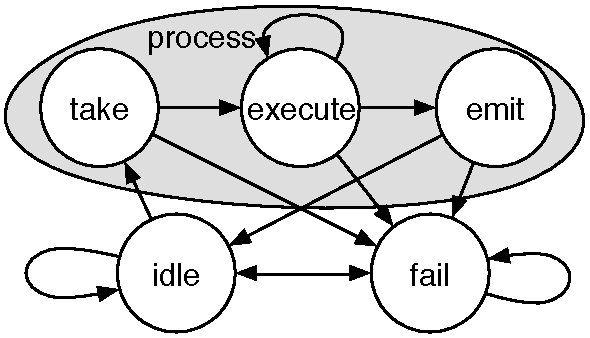
\includegraphics[width=0.7\linewidth]{images/bolt-fsm}
\caption{Finite state automaton describing bolt states.}
\label{figure-fsa}
\end{figure}

%\begin{figure}
%	\centering	
%	\begin{tikzpicture}[->,>=stealth',shorten >=1pt,auto,node distance=2.5cm,semithick, every node/.style={scale=0.55}]
%	
%	\tikzstyle{every state}=[fill=white,text=black,minimum width={width("execute")+10pt}]
%	
%	
%	\node[state]            (I) {$idle$};  
%	\node[state]         (T) [above right of=I] {$take$};  
%	\node[state]         (E) [right of=T] {$execute$};
%	\node[state]         (F) [below right of=I] {$fail$};
%	\node[state]         (EM) [right of=F] {$emit$};
%	
%	\path (I) edge              node {} (T)
%	edge              node {} (F)
%	edge [loop above]  node {} (I)
%	(E) edge [loop right] node {} (E)
%	edge              node {} (EM)
%	(T) edge              node {} (E)
%	edge              node {} (F)
%	(EM) edge             node {} (I)
%	edge              node {} (F)
%	(F) edge [loop below]  node {} (F);
%	edge [bend right]  node {} (I);
%	\end{tikzpicture}
%	\caption{Finite state automaton describing bolt states.}
%	\label{figure-fsa}
%\end{figure}
%To give an idea about how the model is formalized, 
We provide, as an example, one of the formulae defining the processing state. Formula \ref{formula:1} can be read as \textit{``for all bolts: if a bolt j is processing tuples, then it has been processing tuples since it took those tuples from the queue, (or since the origin of the events), and it will keep processing those tuples until it will either emit them or fail. Moreover, the bolt is not in a failure state''.}
\begin{align}
\small
%
\bigwedge_{
	i \in \mathbf{B} } 
\left( 
\begin{array}{l}
\p{i} \Rightarrow \\
\p{i} \, \Snc \, ( \ta{i} \lor (\ori \land \p{i})) \land \\
\p{i} \, \U \, (\e{i} \lor \f{i}) \land \lnot \f{i} 
\end{array}
\right) \label{formula:1} 
%
\end{align}
The number of tuples emitted by a bolt depends on the number of incoming tuples. The ratio $\frac{\#output\_tuples}{\#input\_tuples}$ %is used to 
expresses the ``kind of function''  performed by the bolt and is given as configuration parameter. 
All the emitted tuples are then added to the receive queues of the bolts subscribing to the emitting nodes.
In the same way, whenever a bolt reads tuples from the queue, the number of elements in queue decreases. To this end, formula \ref{formula:2}, imposes that \textit{``if a bolt takes elements from its queue, the number of queued elements in the next time instant will be equal to the current number of elements plus the quantity of tuples being added (emitted) from other connectd nodes minus the quantity of tuples being read''.}
\begin{align}\small
%
\bigwedge_{
	\begin{subarray}{c}
	\,j \in B
	\end{subarray}
} &( \ta{j}{}  \Rightarrow (\aX q_j = q_j + \ra{j} - \rt{j} )) \label{formula:2}
%
\end{align}
These functional constraints are fixed for all the nodes and they are not configurable.
%What is configurable and can be tuned changing the parameters of the model is everything concerning 
The structure of the topology, the parallelism level of each node, the bolt function and the non-functional requirements, as, for example, the time needed for a bolt in order to process a tuple, the minimum and maximum time between failures and the spout emitting rate are configurable parameters of the model.
Currently, the verification tool accepts %as configuration format 
a JSON file containing all the configuration parameters.
OSTIA supports such format and is able to extract from static code analysis a partial set of features, and an almost complete set of parameters after monitoring a short run of the system. The user can complete the JSON file by adding some verification-specific settings.







\section{Evaluation}
%\textbf{@Marcello,Francesco: we should also probably elaborate on the kind of verification technique we are using and how that can help in evaluating the topology.. remember here we do not have the DICE restriction so we can mention any kind of analysis that it would be possible to run, also analyses that are currently in the hands of other DICE partners!!}

%\begin{itemize}
%\item we can use the ATC case study as much as we want - that yields already three topologies that we can infer
%\item ATC has agreed that we can mention their role in this exercise, I also showed them the topology that we elicited basically with OSTIA and they already made considerations on how to improve it
%\item in the evaluation we should also comment on how OSTIA can help you in visualizing the application topology that you may be considering to use by reusing a big-data application for something else... visualising the application topology and analysing it may allow you to improve it while you are using it as a starting point for your application
%\item another application that we can use is the one that NETF is considering for their own scenario, KILLRWEATHER - \url{https://github.com/killrweather/killrweather}
%\item any additional case that we can run?
%\item what do the results show? do we have a way to quickly quantify the time that is saved by using this approach? e.g., the time that is saved in setting up and running the infrastructure and how much would that time saved have costed these could be valuable evaluation insights
%\end{itemize}
We evaluated OSTIA through qualitative evaluation and case-study research featuring an open-/closed-source industrial case study (see Section \ref{cs}) and two open-source case studies (see Section \ref{os}) on which we also applied complex formal verification (see Section \ref{ver}).

\subsection{Industrial Case-Study}\label{cs}

%As previously introduced in Section \ref{ra}, 
OSTIA was evaluated using several topologies part of the SocialSensor App. Our industrial partner is having
performance and availability outages connected to currently unknown
circumstances. Therefore, the objective of our evaluation for OSTIA was twofold:
(a) allow our industrial partner to enact architecture refactoring of their
application with the goal of discovering any patterns or hotspots that may be
requiring further architectural reasoning; (b) understand whether OSTIA provided
valuable feedback helping designers in tuning their application through a design-and-refactor loop.%to endure the continuous architecting exercise.


In addition to formal verification, specific algorithms for graph analysis can be integrated in OSTIA to offer a deeper insight of the applications.
For instance, the industrial case study has been analyzed with two algorithms to identify linear sequences of nodes and clusters in the topology graph.
Topology linearisation results in sorting the processing elements in a topology in a way that topology looks more linear, visually. 
This step ensures that visual investigation and evaluation of the structural complexity of the topology is possible by direct observation. 
Topology clustering implies identifying coupled processing elements (i.e., bolts and spouts) and cluster them together (e.g., by means of graph-based analysis) in a way that elements in a cluster have high cohesion and loose-coupling with elements in other clusters. 
Simple clustering or Social-Network Analysis mechanisms can be used to infer clusters. 
Clusters may require, in general, additional attention since they could turn out to become bottlenecks. 
Reasoning more deeply on clusters and their resolution may lead to establishing the Storm scheduling policy best-fitting with the application.


OSTIA standard output\footnote{Output of OSTIA analyses is not evidenced for the
sake of space.} for the smallest of the three SocialSensor topologies, namely
the ``focused-crawler" topology, is outlined in Fig. \ref{topo1}.

\begin{figure*}
\begin{center}
		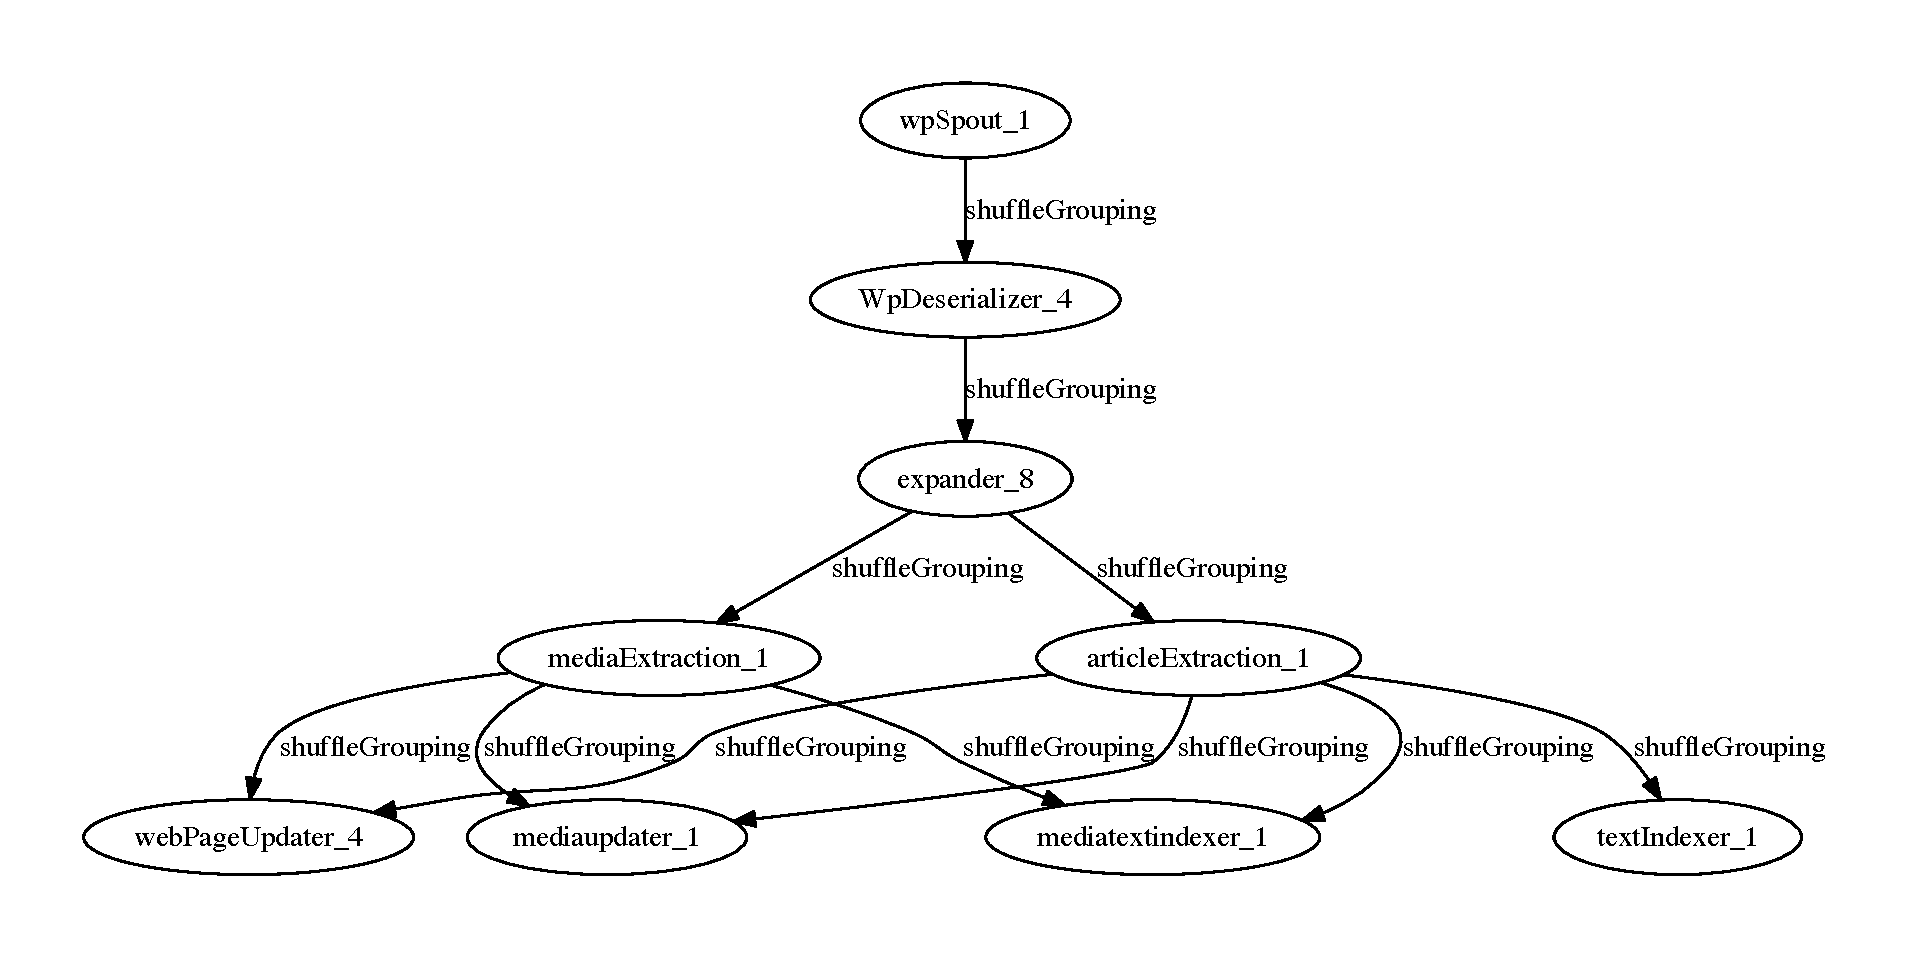
\includegraphics[width=11cm]{images/output/focused_crawler}
		\caption{SocialSensor App, OSTIA sample output partially linearised (top) and cascaded (bottom left and right).}
		\label{topo1}
		\end{center}
\end{figure*}



%OSTIA has been proved particularly helpful in visualising the complex topologytogether with the parallelism level of each components. 


%REMOVED MOVED TO CASE-STUDY ANALYSIS 
%\subsubsection{Topology clustering}\label{3}
%Topology clustering is outlined in Fig. \ref{fig:clustering}. Topology clustering implies identifying coupled processing elements (i.e., bolts and spouts) and cluster them together (e.g., by means of graph-based analysis) in a way that elements in a cluster have high cohesion and loose-coupling with elements in other clusters. Simple clustering or Social-Network Analysis mechanisms can be used to infer clusters. These clusters may require additional attention since they could turn out to become bottlenecks. Reasoning more deeply on clusters and their resolution may lead to establishing the Storm scheduling policy best-fitting with the application. We will elaborate on this in Section \ref{sec:performance-boosting}.
%%\emph{\bf Does it relates with Storm scheduling?}
%
%\begin{figure}
%	\begin{center}
%		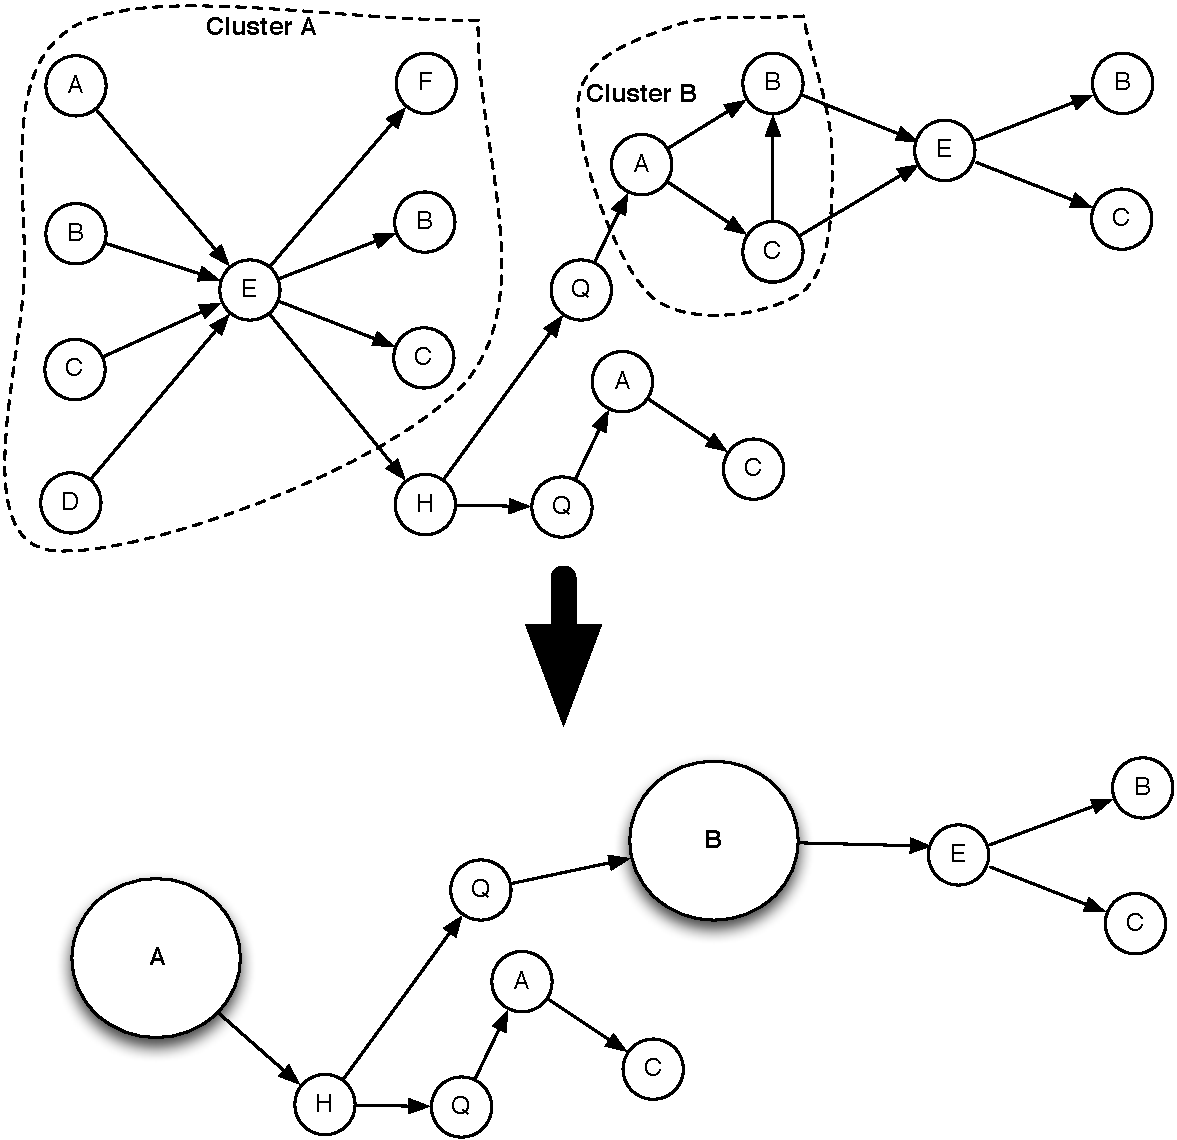
\includegraphics[width=6.5cm]{images/clustering}
%		\caption{clustering.}
%		\label{fig:clustering}
%	\end{center}
%\end{figure}


%REMOVED MOVED TO CASE-STUDY ANALYSIS 
%\subsubsection{Linearising a topology}\label{4}
%
%Topology linearisation is outlined in Fig. \ref{fig:linearizing}. Sorting the processing elements in a topology in a way that topology looks more linear, visually. This step ensures that visual investigation and evaluation of the structural complexity of the topology is possible by direct observation. It is sometimes essential to provide such a visualisation to evaluate how to refactor the topology as needed.

%\begin{figure}
%	\begin{center}
%		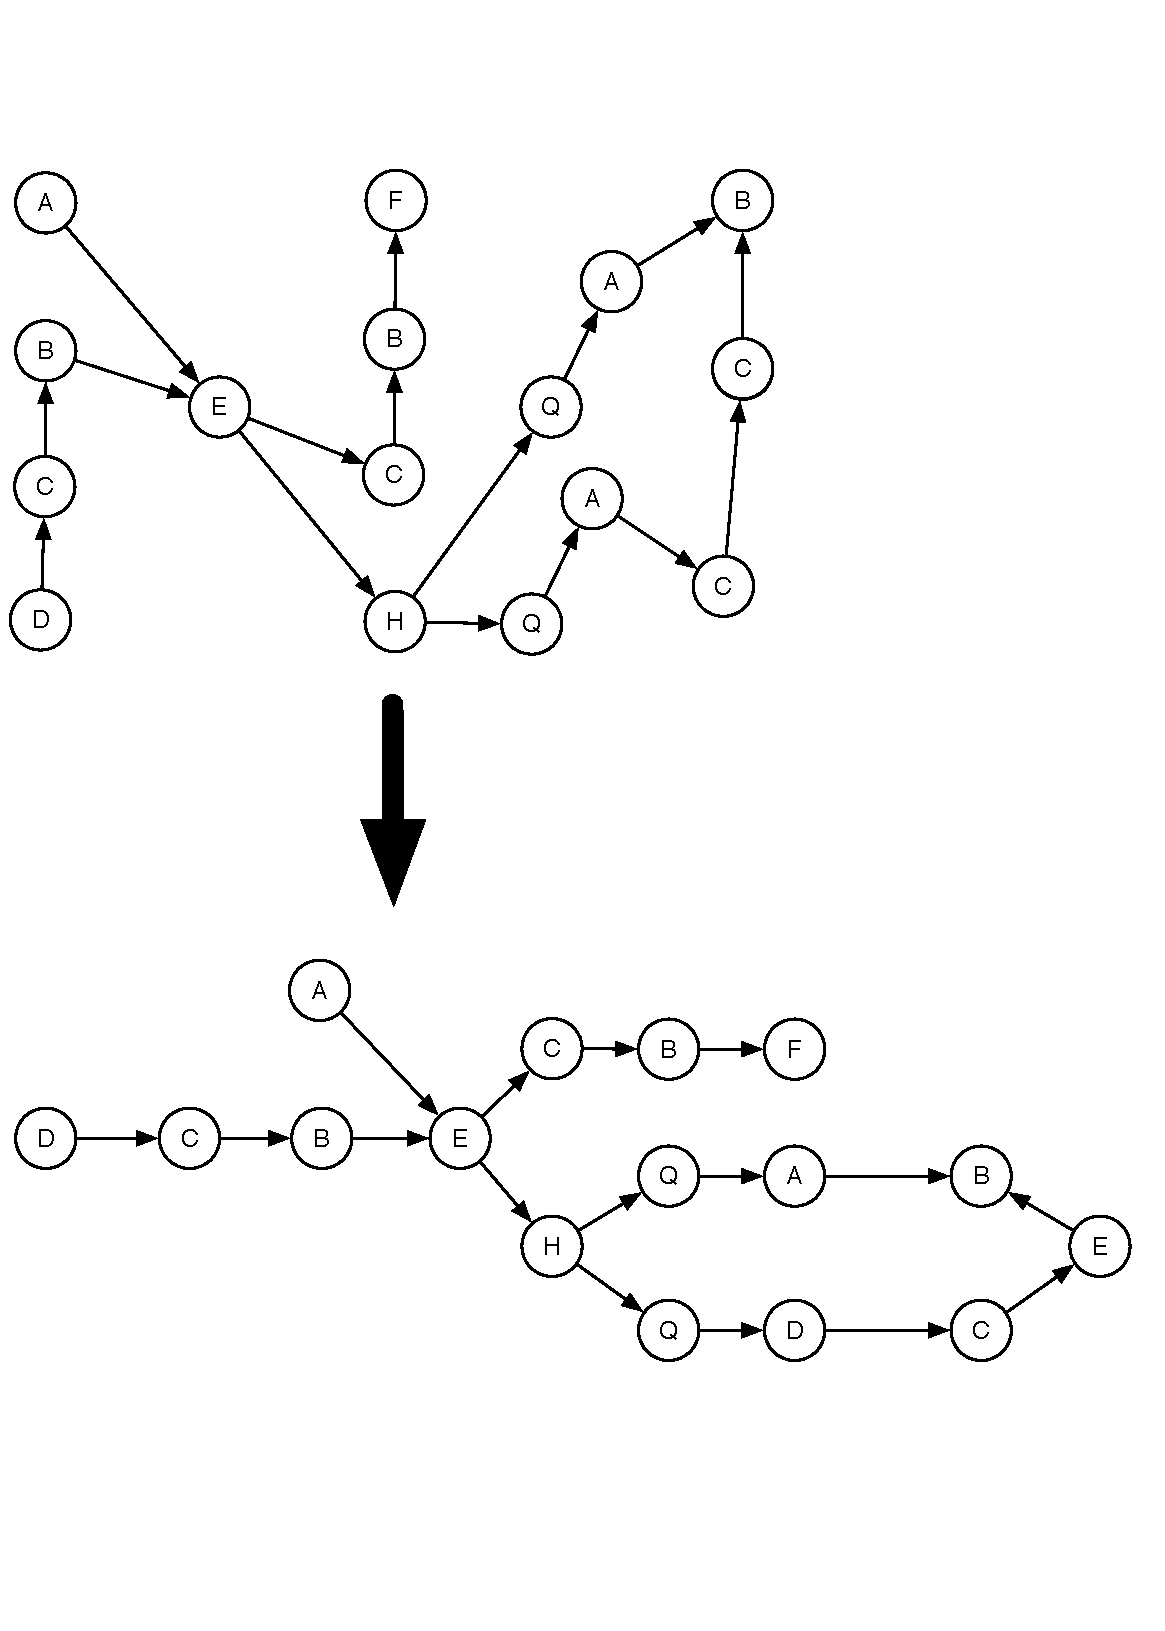
\includegraphics[width=5cm]{images/linearizing}
%		\caption{linearising.}
%		\label{fig:linearizing}
%	\end{center}
%\end{figure}



Combining this
information with runtime data (i.e., latency times) our industrial partner observed
that the ``expander" bolt needed additional architectural reasoning. More in particular, the bolt in question concentrates a lot of the topology's progress on its queue, greatly hampering the topology's scalability. In our partner's scenario, the limited scalability was blocking the expansion of the topology in question with more data sources and sinks.
In addition, the partner welcomed the idea of using OSTIA as a mechanism to enact the refactoring of the topology in question as part of the needed architectural
reasoning.
%\comment{for example? elaborate more on this. the reviewers will likely say its vague...}

Besides this pattern-based evaluation and assessment, OSTIA algorithmic analyses\todoMB{}{Non mi è chiaro quali siano le analisi oltre ai pattern...}
assisted our client in understanding that the topological structure of the
SocialSensor app would be better fit for batch processing rather than streaming,
since the partner observed autonomously that too many database-output spouts and
bolts were used in their versions of the SocialSensor topologies. In so doing,
the partner is now using OSTIA to drive the refactoring exercise towards a
Hadoop Map Reduce~\cite{hadoop}
%\footnote{\url{http://hadoop.apache.org/}} 
framework for batch processing.

%\comment{this section is not good enough, we require to add more information, for example what would be the target architecture after refactoring looks like? we said some patters were idenfitified but we didnt say details of continuous rearchitecting...and also formal verification process for this}

\begin{figure}
\begin{center}
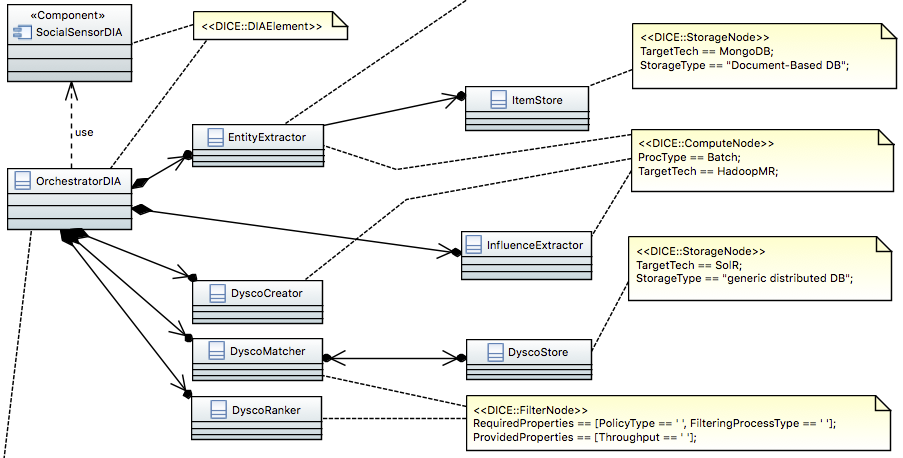
\includegraphics[width=8cm]{images/atc}
		\caption{Industrial case-study, a refactored architecture.}
		\label{atc}
		\end{center}
\end{figure}

As a followup of our analysis, our partner is refactoring his own high-level software architecture adopting a lambda-like software architecture style \cite{lambda} (see Fig. \ref{atc}) which includes the Social-Sensor App (Top of Fig. \ref{atc}) as well as several additional computation components. In summary, the refactoring resulting from OSTIA-based analysis equated to deferring part of the computations originally intended in the expander bolt part of the Storm topology within the Social Sensor app to additional ad-hoc Hadoop Map Reduce jobs with similar purpose (e.g., the EntityExtractor compute node in Fig. \ref{atc}) and intents but batched out of the topological processing in Storm (see Fig. \ref{atc})\footnote{several other overburdened topological elements were refactored but were omitted here due to industrial secrecy}. 

Our qualitative evaluation of the refactored architecture by means of several interviews and workshops revealed very encouraging results. 
%However, we are yet to quantitatively evaluate whether the new software architecture actually reflects a tangible boost in terms of performance and scalability.\todoMB{}{Azz...pesante questa...}

\subsection{Evaluation on Open-Source Software}\label{os}

To confirm the usefulness and capacity of OSTIA to enact a continuous
architecting cycle, we applied it in understanding (first) and attempting
improvements of two open-source applications, namely, the previously introduced
DigitalPebble~\cite{digitalpebble} and 
%\footnote{\url{https://github.com/DigitalPebble}} and
StormCV~\cite{stormCV}
%\footnote{\url{https://github.com/sensorstorm/StormCV}}
applications. Figures \ref{dp} and \ref{scv} outline standard OSTIA output for the two applications. Note that we did not have any prior knowledge concerning the two applications in question and we merely run OSTIA on the applications' codebase dump in our own experimental machine. OSTIA output takes mere seconds for small to medium-sized topologies (e.g., around 25 nodes). 
%
\begin{figure}
\begin{center}
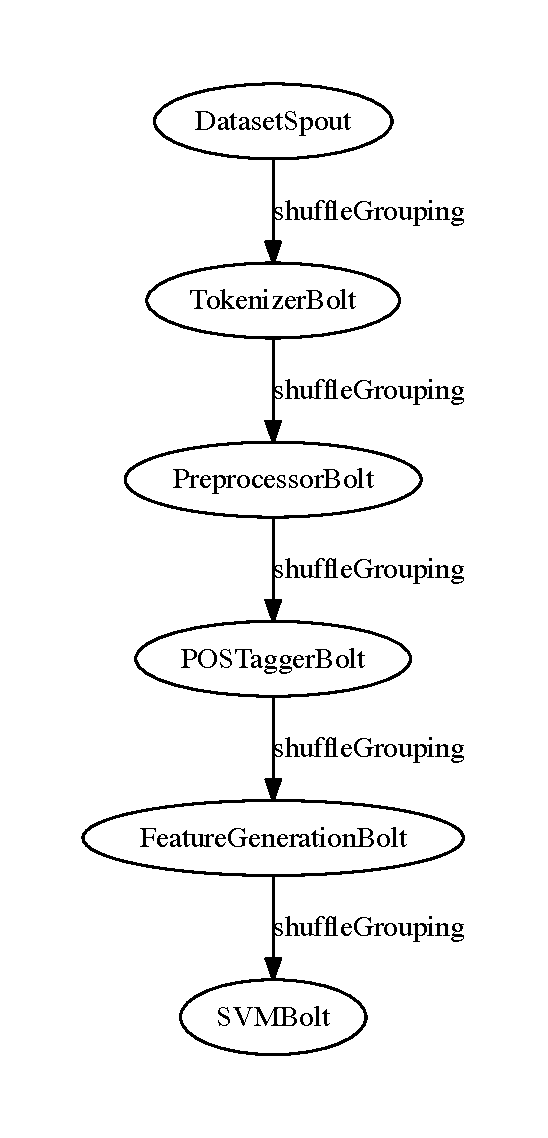
\includegraphics[width=4cm]{images/output/senti_storm}
		\caption{StormCV topology (linearised).}
		\label{scv}
		\end{center}
\end{figure}
%%%%
%%%%\begin{figure}
%%%%\label{fig:oscasestudy}
%%%%\centering 
%%%%\subfigure[{\footnotesize DigitalPebble topology.}]{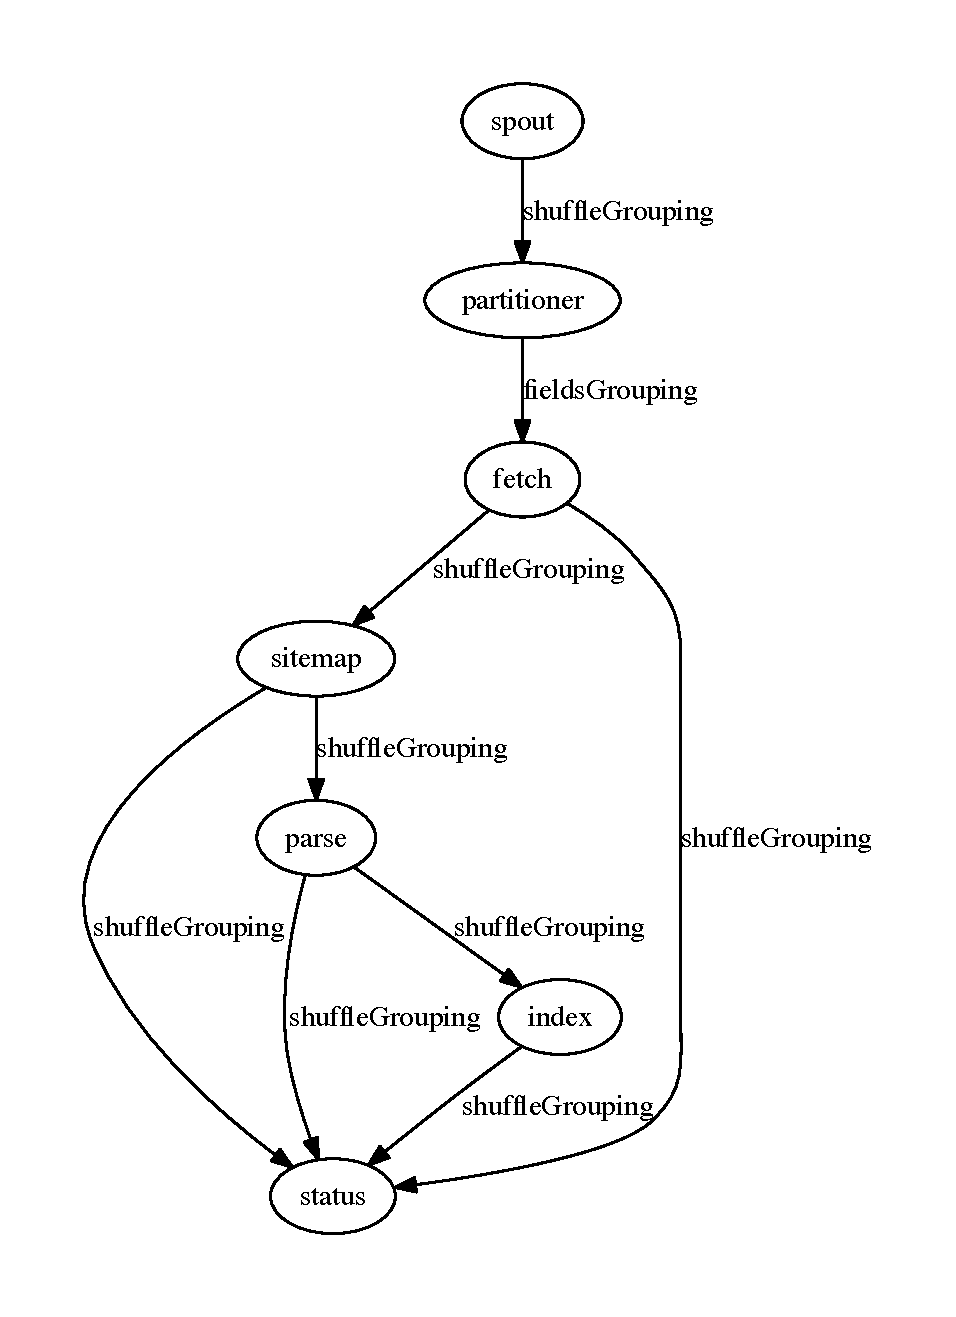
\includegraphics[width=4.5cm]{images/output/crawl}}\label{dp}
%%%%\hspace{0.5cm}
%%%%\subfigure[{\footnotesize StormCV topology.}]{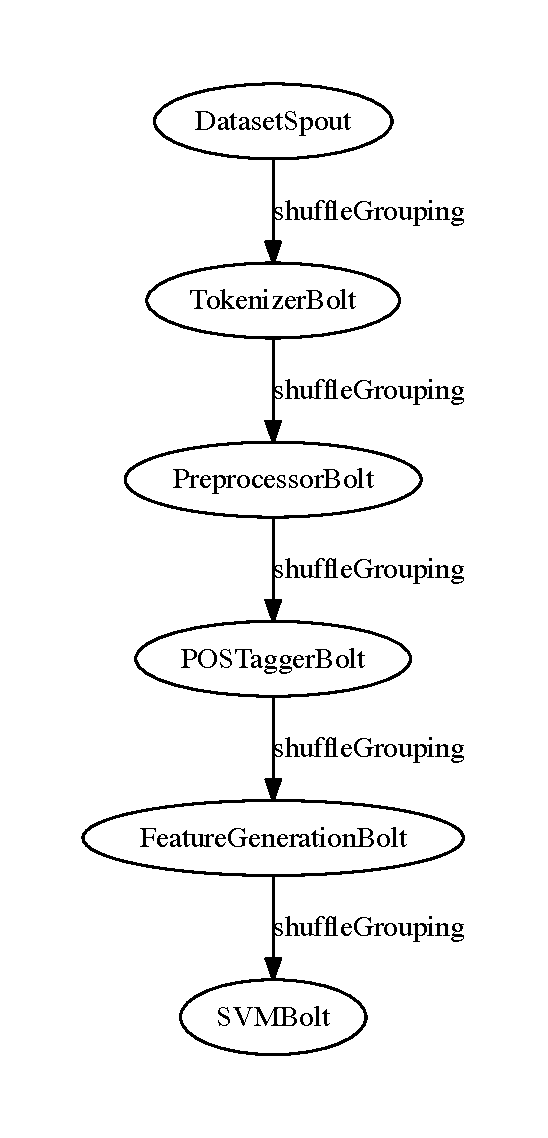
\includegraphics[width=3cm]{images/output/senti_storm}}\label{scv}
%%%%\end{figure}

The OSTIA output aided as follows: (a) the output summarised in Fig. \ref{dp}
allowed us to immediately grasp the functional behavior of the DigitalPebble and
StormCV topologies allowing us to interpret correctly their operations before
reading long documentation or inspecting the code; (b) OSTIA aided us in visually interpreting the complexity of the applications at hand; (c) OSTIA allowed us to spot several anti-patterns in the DigitalPebble Storm application around the ``sitemap" and ``parse" bolts, namely, a multiple cascading instance of the multi-anchoring pattern and a persistent-data pattern. Finally, OSTIA aided in the identification of the computational funnel anti-pattern around the "status" bolt closing the DigitalPebble topology. With this evaluation at hand, developers in the respective communities of DigitalPebble and StormCV could refactor their topologies, e.g., aided by OSTIA-based formal verification that proves the negative effects of said anti-patterns.
%
%\comment{this section needs further elaboration. we need to elaborate our discussion to visually locate these anti patterns.}
% \comment{you said first, where is the second? this is incomplete}
%
%\begin{figure}
%\begin{center}
%		\includegraphics[width=2.7cm]{}
%		\caption{}
%		\label{scv}
%\end{center}
%\end{figure}

\subsection{OSTIA-based Formal Verification: An Industrial Case-Study}

In this section we outline the results from OSTIA-based formal verification applied on (one of) the topologies used by our industrial partner in practice. 
Results provide valuable insights for improving these topologies through refactoring.

\begin{figure}
\begin{center}
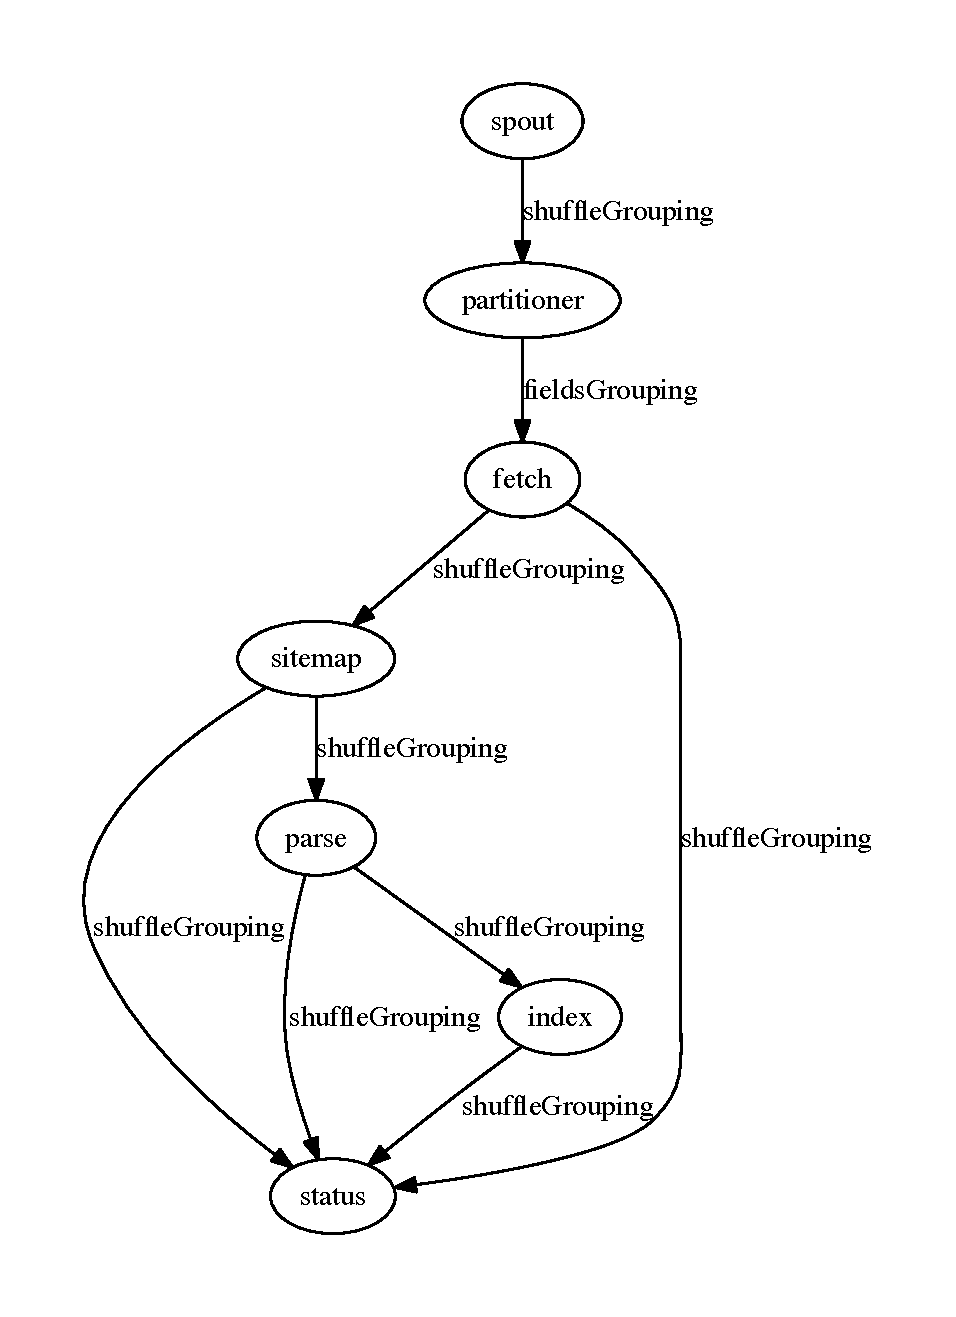
\includegraphics[width=6cm]{images/output/crawl}
		\caption{DigitalPebble topology.}
		\label{dp}
		\end{center}
\end{figure}
The formal analysis of the ``focused-crawler'' topology confirmed the critical role of the ``expander'' bolt, previously noticed with the aim of OSTIA visual output. It emerged from the output traces that there exists an execution of the system, even without failures, where the queue occupation level of the bolt is unbounded. Figure~\ref{verif-trace} shows how the tool constructed a periodic model in which a suffix (highlighted by the gray background) of a finite sequence of events is repeated infinitely many times after a prefix (on white background). After ensuring that the trace is not a spurious model, we concluded that the expander queue, having an increasing trend in the suffix, is unbounded. 
As shown in the the output trace at the bottom of Fig.~\ref{verif-trace}, further analyses on the DigitalPebble use case revealed that the same problem affects the ``status'' bolt of the DigitalPebble topology. This finding from the formal verification tool reinforced the outcome of the anti-pattern module of OSTIA, showing how the presence of the computational funnel anti-pattern could lead to an unbounded growth in the queue of the ``status'' bolt.
These types of heavyweight and powerful analyses are made easier by OSTIA in that our tool provides a ready-made analyzable models of the topologies making almost invisible the formal verification layer (other than manually setting and tuning operational parameters for verification). %on top of which OSTIA support is harnessed.
%
%\comment{discuss thge benefit of this, was it possible without formal verification?  elaborate more}
% alternative
%This feedback persuaded to 

\begin{figure}
\centering
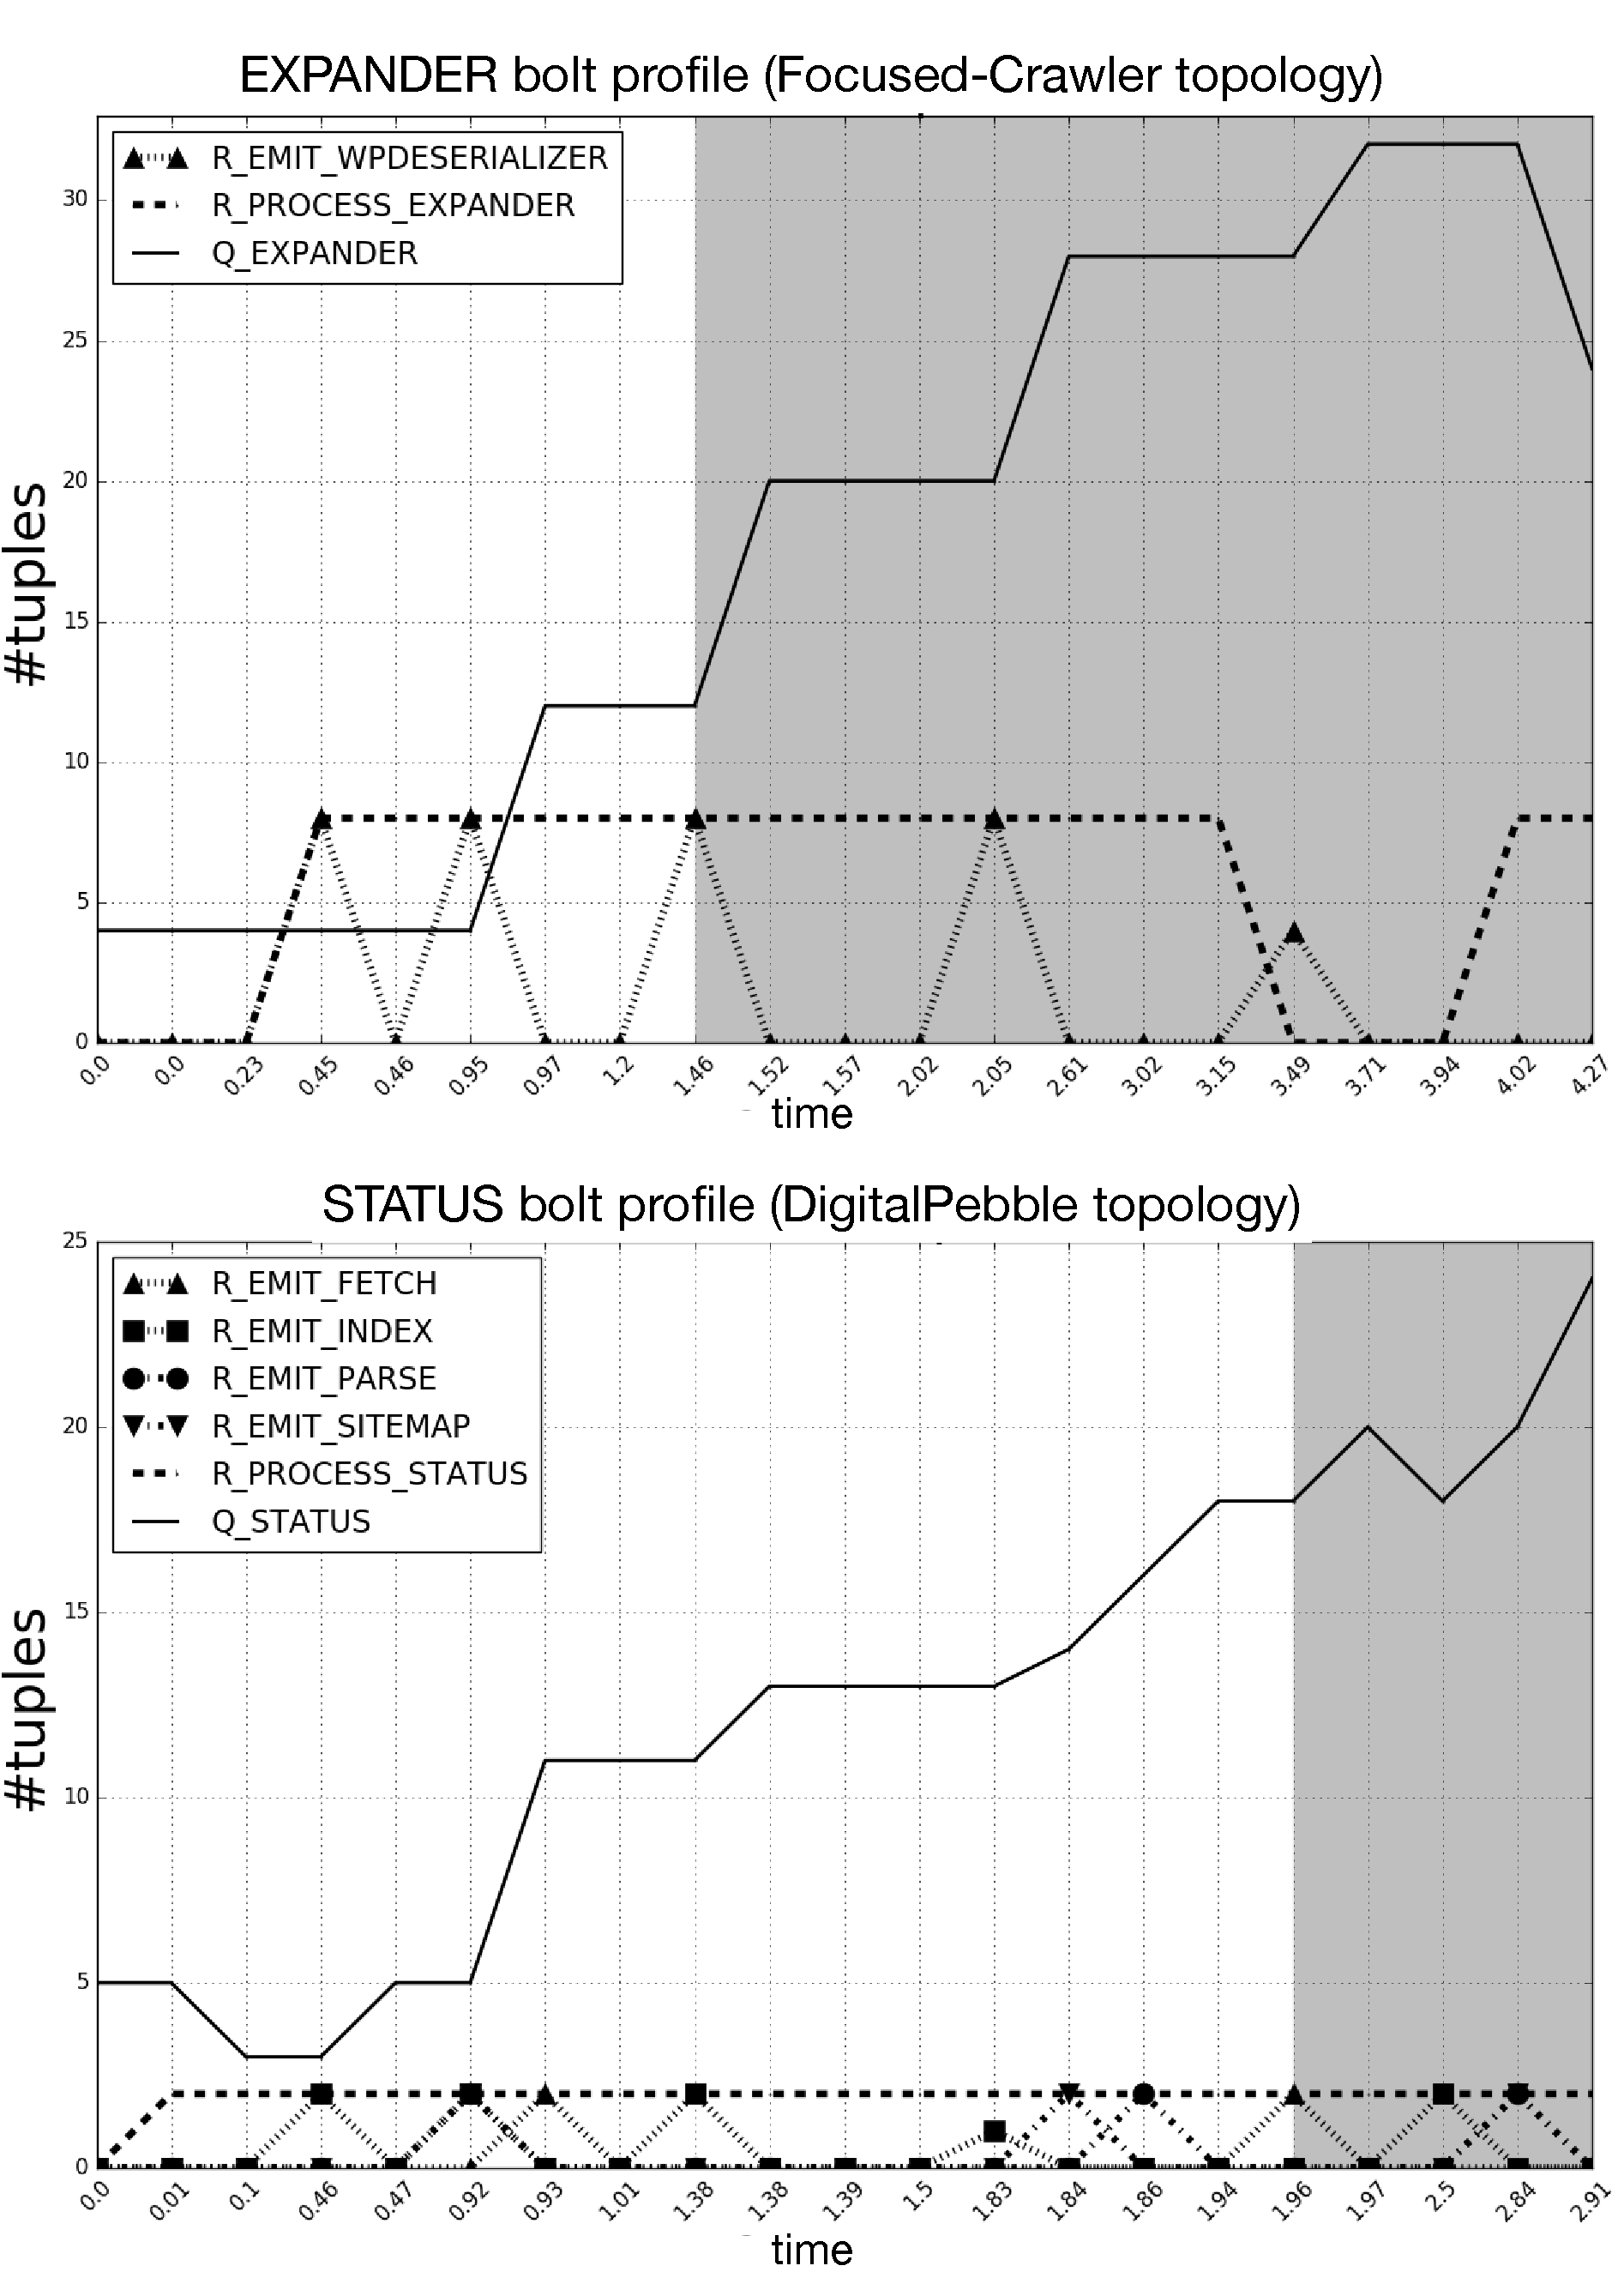
\includegraphics[width=1\linewidth]{images/verif-traces-bw}
\caption{OSTIA-based formal verification output traces showing the evolution of the two bolts over time. Queue trends are displayed as solid black line. Dashed lines show the processing activity of the bolts, while the other lines illustrate the incoming tuples from the subscribed nodes (\texttt{emit} events).}
\label{verif-trace}
\end{figure}

\label{eval}

\section{Discussion}
% no \IEEEPARstart
This section discusses some findings and the limitations of OSTIA.

\subsection{Findings and Continuous Architecting Insights}

OSTIA represents one humble, but significant step at supporting practically the necessities behind developing and maintaining high-quality big-data application architectures. In designing and developing OSTIA we encountered a number of insights that may aid continuous architecting.

First, we found (and observed in industrial practice) that it is often more useful to develop a quick-and-dirty but ``runnable" architecture topology than improving the topology at design time for a tentatively perfect execution. This is mostly the case with big-data applications that are developed stemming from previously existing topologies or applications. OSTIA hardcodes this way of thinking by supporting reverse-engineering and recovery of deployed topologies for their incremental improvement. Such improvement is helpful because these topologies running continuously on rented clusters and the refactoring can help in boosting the performance and therefore requiring less resources and less cost for the rented clusters. Although we did not carry out extensive qualitative or quantitative evaluation of OSTIA in this regard, we are planning additional industrial experiments for future work with the goal of increasing OSTIA usability and practical quality.

Second, big-data applications design is an extremely young and emerging field for which not many software design patterns have been discovered yet. The (anti-)patterns and approaches currently hardcoded into OSTIA are inherited from related fields, e.g., pattern- and cluster-based graph analysis. Nevertheless, OSTIA may also be used to investigate the existence of recurrent and effective design solutions (i.e., design patterns) for the benefit of big-data application design. We are improving OSTIA in this regard by experimenting on two fronts: (a) re-design and extend the facilities with which OSTIA supports anti-pattern detection; (b) run OSTIA on multiple big-data applications stemming from multiple technologies beyond Storm (e.g., Apache Spark, Hadoop Map Reduce, etc.) with the purpose of finding recurrent patterns. A similar approach may feature OSTIA as part of architecture trade-off analysis campaigns \cite{atam}.

Third, a step which is currently undersupported during big-data applications design is devising an efficient algorithmic breakdown of a workflow into an efficient topology. Conversely, OSTIA does support the linearisation and combination of multiple topologies, e.g., into a cascade. Cascading and similar super-structures may be an interesting investigation venue since they may reveal more efficient styles for big-data architectures beyond styles such as Lambda Architecture \cite{lambda} and Microservices \cite{balalaie2016microservices}. OSTIA may aid in this investigation by allowing the interactive and incremental improvement of multiple (combinations of) topologies together.

\subsection{Approach Limitations and Threats to Validity}\label{lim}

Although OSTIA shows promise both conceptually and as a practical tool, it shows several limitations.

First of all, OSTIA only supports only a limited set of DIA middleware technologies. Multiple other big-data frameworks such as Apache Spark, Samza, exist to support both streaming and batch processing. 

Second, OSTIA only allows to recover and evaluate previously-existing topologies, its usage is limited to design improvement and refactoring phases rather than design. Although this limitation may inhibit practitioners from using our technology, the (anti-)patterns and algorithmic approaches elaborated in this paper help designers and implementors to develop the reasonably good-quality and ``quick" topologies upon which to use OSTIA for continuous improvement.

Third, OSTIA does offer essential insights to aid deployment as well (e.g., separating or \emph{clustering} complex portions of a topology so that they may run on dedicated infrastructure) and therefore the tool may serve for the additional purpose of aiding deployment design. However, our tool was not designed to be used as a system that aids deployment planning and infrastructure design. Further research should be invested into combining on-the-fly technology such as OSTIA with more powerful solvers that determine infrastructure configuration details and similar technological tuning, e.g., the works by Peng et Al. \cite{PengGWRYC14} and similar.
%Rather, as specified previously in the introduction, OSTIA was meant to evaluate and increase the quality of topologies \emph{before} they enter into operation since the continuous improvement cycles connected to operating the topology and learning from operation are often costly and still greatly inefficient. \comment{but we provided evidences that we exploit the operation data for formal verification and performance improvements. this paragraph is a bit vague, please edit}

Fourth, although we were able to discover a number of recurrent anti-patterns to be applied during OSTIA analysis, we were not able to implement all of them in practice and in a manner which allows to spot both the anti-pattern and any problems connected with it. For example, detecting the ``Cycle-in topology" is already possible, however, OSTIA would not allow designers to understand the consequence of the anti-pattern, i.e., where in the infrastructure do the cycles cause troubles. Also, there are several features that are currently under implementation but not released within the OSTIA codebase, for example, the ``Persistent Data" and the ``Topology Cascading" features.

In the future we plan to tackle the above limitations furthering our understanding of streaming design as well as the support OSTIA offers to designers during continuous architecting.

\label{disc}



\section{Previous and Related Work}
% no \IEEEPARstart
%\begin{itemize}
%\item mention DICE
%\item mention work by Len Bass on Big-Data
%\item other stuff on big data?
%\item feel free to extend this section with Previous work of course :)
%\end{itemize}

The work behind OSTIA stems from the EU H2020 Project called DICE\footnote{\url{http://www.dice-h2020.eu/}} where we are investigating the use of model-driven facilities to support the design and quality enhancement of Big-Data applications. Much similarly to the DICE effort, the IBM Stream Processing Language (SPL) initiative \cite{ibmspl} provides an implementation language specific to programming streams management (e.g., Storm jobs) and related reactive systems based on the Big-Data paradigm. 

In addition, there are several work close to OSTIA in terms of their foundations and type of support. 

First, from a quantitative perspective, much literature discusses quality analyses of Storm topologies, e.g., from a performance~\cite{perfbd} or reliability point of view \cite{bigdatareliab}. Said works use complex math-based approaches to evaluating a number of Big data architectures, their structure and general configuration. However, although novel, these approaches do not suggest any significant design improvement method or pattern to make the improvements \emph{deployable}. With OSTIA, we make available a tool that automatically elicits a Storm topology and, while doing so, analyses said topology to evaluate it against a number of consistency checks that make the topology consistent with the framework it was developed for (Storm, in our case). To the best of our knowledge, no such tool exists to date. 

Second, from a modelling perspective, approaches such as StormGen~\cite{stormgen} offer means to develop Storm topologies in a model-driven fashion using a combination of generative techniques based on XText and heavyweight (meta-)modelling, based on EMF, the standard Eclipse Modelling Framework Format. Although the first of its kind, StormGen merely allows the specification of a Storm topology, without applying any consistency checks or without offering the possibility to \emph{recover} said topology once it has been developed. By means of OSTIA, designers and developers can work hand in hand while refining their Storm topologies, e.g., as a consequence of verification or failed checks through OSTIA. Tools such as StormGen can be used to assist preliminary development of quick-and-dirty Storm topologies.
%Fourth, from a verification perspective, no previous effort tried yet to combine formal verification and architectural modelling of streaming topologies. Our attempt serves as a first rudimentary effort towards using complex and valuable verification approaches in combination with lightweight and agile DevOps inspired tools and approaches.
%%...\\
%%\textbf{@Marcello,Francesco: here we should probably elaborate on what kind of verification approach we are using and what other verifications may be done, e.g., using some related work at this point... e.g., is there any other verification attempt considering JSON as an interchange format? I would discuss these and compare them to OSTIA as a whole}
%=======
%\textbf{@Marcello,Francesco: here we should probably elaborate on what kind of verification approach we are using and what other verifications may be done, e.g., using some related work at this point... e.g., is there any other verification attempt considering JSON as an interchange format? I would discuss these and compare them to OSTIA as a whole}\\

Third, from a verification perspective, to the best of our knowledge, this represents the first attempt to build a formal model representing Storm topologies, and the first try in making a configurable model aiming at running verification tasks of non-functional properties for big data applications. While some works concentrate on exploiting big data technologies to speedup verification tasks~\cite{camilli2014}, others focus on the formalization of the specific framework, but remain application-independent, and their goal is rather to verify properties of the framework, such as reliability and load balancing~\cite{dicomputational}, or the validity of the messaging flow in MapReduce~\cite{yang2010formalizing}\footnote{The Authors' work is partially supported by the European Commission grant no. 644869 (EU H2020), DICE. Also, Damian's work is partially supported by the European Commission grant no. 610531 (FP7 ICT Call 10), SeaClouds.}.
%
%.
%
%Finally, several deployment modelling technologies may be related to OSTIA since their role is to model the deployment structure for Big data architectures such as in Celar\footnote{\url{https://github.com/CELAR/c-Eclipse}}, that is, a deployment modelling technology based on the TOSCA OASIS Standard\footnote{\url{https://www.oasis-open.org/apps/org/workgroup/tosca/}}. Celar may be used together with OSTIA In a scenario where OSTIA helps architecture refinement in function of infrastructure needs/requirements
\label{rw}



% An example of a floating figure using the graphicx package.
% Note that \label must occur AFTER (or within) \caption.
% For figures, \caption should occur after the \includegraphics.
% Note that IEEEtran v1.7 and later has special internal code that
% is designed to preserve the operation of \label within \caption
% even when the captionsoff option is in effect. However, because
% of issues like this, it may be the safest practice to put all your
% \label just after \caption rather than within \caption{}.
%
% Reminder: the "draftcls" or "draftclsnofoot", not "draft", class
% option should be used if it is desired that the figures are to be
% displayed while in draft mode.
%
%\begin{figure}[!t]
%\centering
%\includegraphics[width=2.5in]{myfigure}
% where an .eps filename suffix will be assumed under latex, 
% and a .pdf suffix will be assumed for pdflatex; or what has been declared
% via \DeclareGraphicsExtensions.
%\caption{Simulation results for the network.}
%\label{fig_sim}
%\end{figure}

% Note that the IEEE typically puts floats only at the top, even when this
% results in a large percentage of a column being occupied by floats.


% An example of a double column floating figure using two subfigures.
% (The subfig.sty package must be loaded for this to work.)
% The subfigure \label commands are set within each subfloat command,
% and the \label for the overall figure must come after \caption.
% \hfil is used as a separator to get equal spacing.
% Watch out that the combined width of all the subfigures on a 
% line do not exceed the text width or a line break will occur.
%
%\begin{figure*}[!t]
%\centering
%\subfloat[Case I]{\includegraphics[width=2.5in]{box}%
%\label{fig_first_case}}
%\hfil
%\subfloat[Case II]{\includegraphics[width=2.5in]{box}%
%\label{fig_second_case}}
%\caption{Simulation results for the network.}
%\label{fig_sim}
%\end{figure*}
%
% Note that often IEEE papers with subfigures do not employ subfigure
% captions (using the optional argument to \subfloat[]), but instead will
% reference/describe all of them (a), (b), etc., within the main caption.
% Be aware that for subfig.sty to generate the (a), (b), etc., subfigure
% labels, the optional argument to \subfloat must be present. If a
% subcaption is not desired, just leave its contents blank,
% e.g., \subfloat[].


% An example of a floating table. Note that, for IEEE style tables, the
% \caption command should come BEFORE the table and, given that table
% captions serve much like titles, are usually capitalized except for words
% such as a, an, and, as, at, but, by, for, in, nor, of, on, or, the, to
% and up, which are usually not capitalized unless they are the first or
% last word of the caption. Table text will default to \footnotesize as
% the IEEE normally uses this smaller font for tables.
% The \label must come after \caption as always.
%
%\begin{table}[!t]
%% increase table row spacing, adjust to taste
%\renewcommand{\arraystretch}{1.3}
% if using array.sty, it might be a good idea to tweak the value of
% \extrarowheight as needed to properly center the text within the cells
%\caption{An Example of a Table}
%\label{table_example}
%\centering
%% Some packages, such as MDW tools, offer better commands for making tables
%% than the plain LaTeX2e tabular which is used here.
%\begin{tabular}{|c||c|}
%\hline
%One & Two\\
%\hline
%Three & Four\\
%\hline
%\end{tabular}
%\end{table}


% Note that the IEEE does not put floats in the very first column
% - or typically anywhere on the first page for that matter. Also,
% in-text middle ("here") positioning is typically not used, but it
% is allowed and encouraged for Computer Society conferences (but
% not Computer Society journals). Most IEEE journals/conferences use
% top floats exclusively. 
% Note that, LaTeX2e, unlike IEEE journals/conferences, places
% footnotes above bottom floats. This can be corrected via the
% \fnbelowfloat command of the stfloats package.




\section{Conclusion}
%Applications that make heavy use of big data application frameworks require intensive reasoning of the system architecture. 
We set out to assist the continuous architecting of big data streaming designs by OSTIA, a toolkit to assist designers and developers to facilitate static analysis of the architecture and provide automated constraint verification in order to identify design anti-patterns and provide structural refactorings. OSTIA helps designers and developers by recovering and analysing the architectural topology on-the-fly, assisting them in: (a) reasoning on the topological structure and how to refine it; (b) export the topological structure consistently with restrictions of their reference development framework so that further analysis (e.g., formal verification) may ensue. In addition, while performing on-the-fly architecture recovery, the analyses that OSTIA is able to apply focus on checking for the compliance to essential consistency rules specific to targeted big data frameworks. Finally, OSTIA allows to check whether the recovered topologies contain occurrences of key anti-patterns. By running a case-study with a partner organization, we observed that OSTIA assists designers and developers in establishing and continuously improving the quality of topologies behind their big data applications. We confirmed this result running OSTIA on several open-source applications featuring streaming technologies. We released OSTIA as an open-source software~\cite{ostia}. % \url{https://github.com/maelstromdat/OSTIA}. 
 
In the future we plan to further elaborate the anti-patterns, 
%that may emerge across big data topologies 
exploiting graphs analysis techniques inherited from social-networks analysis. Also, we plan to expand OSTIA to support further technologies beyond the most common application framework for streaming, i.e., Storm. Finally, we plan to further evaluate OSTIA using empirical evaluation.

{\small\subsubsection*{Acknowledgment} The Authors' work is partially supported by the European Commission grant no. 644869 (EU H2020), DICE. Also, Damian's work is partially supported by the European Commission grant no. 610531 (FP7 ICT Call 10), SeaClouds.}

{\small\subsubsection*{Appendix} Please follow the link to navigate to the appendices: \url{http://tinyurl.com/zco4sdz}.}\label{conc}




% conference papers do not normally have an appendix


% use section* for acknowledgment
\section*{Acknowledgment}
The Authors' work is partially supported by the European Commission grant no. 644869 (EU H2020), DICE. Also, Damian's work is partially supported by the European Commission grant no. 610531 (FP7 ICT Call 10), SeaClouds.

% trigger a \newpage just before the given reference
% number - used to balance the columns on the last page
% adjust value as needed - may need to be readjusted if
% the document is modified later
%\IEEEtriggeratref{8}
% The "triggered" command can be changed if desired:
%\IEEEtriggercmd{\enlargethispage{-5in}}

% references section

% can use a bibliography generated by BibTeX as a .bbl file
% BibTeX documentation can be easily obtained at:
% http://mirror.ctan.org/biblio/bibtex/contrib/doc/
% The IEEEtran BibTeX style support page is at:
% http://www.michaelshell.org/tex/ieeetran/bibtex/
\bibliographystyle{IEEEtran}
\bibliography{ostia}

% <OR> manually copy in the resultant .bbl file
% set second argument of \begin to the number of references
% (used to reserve space for the reference number labels box)
%\begin{thebibliography}{1}
%
%\bibitem{IEEEhowto:kopka}
%H.~Kopka and P.~W. Daly, \emph{A Guide to \LaTeX}, 3rd~ed.\hskip 1em plus
%  0.5em minus 0.4em\relax Harlow, England: Addison-Wesley, 1999.
%
%\end{thebibliography}




% that's all folks
\end{document}


